%% ============================ Classic wp ===================================
\documentclass[11pt]{article}

% ------------------------- Page and paragraph layout ------------------------
\usepackage[a4paper]{geometry}
\geometry{verbose,tmargin=1in,bmargin=1in,lmargin=1in,rmargin=1in}
%\setcounter{secnumdepth}{-2}
%\setcounter{tocdepth}{-2}
\usepackage{setspace}
\onehalfspacing
%\doublespacing
\setlength{\parindent}{2.75em}
\setlength{\parskip}{1em}
%\renewcommand{\baselinestretch}{1.5}
\usepackage{titlesec}
\titlespacing{\section}{0pt}{1.5ex}{-1.5ex}
\titlespacing{\subsection}{0pt}{1.5ex}{-1.5ex}
\titlespacing{\subsubsection}{0pt}{1.5ex}{-1.5ex}
%\makeatletter
%\renewcommand{\@seccntformat}[1]{}
%\makeatother

%% -------------------------- Info on authors --------------------------------
\usepackage{authblk}

%% --------------------------- Text style ------------------------------------
\usepackage{color}

%% ----------------------------- Endnote -------------------------------------
%\usepackage{endnotes}
%\let\footnote=\endnote

%% -------------------------------- Fonts ------------------------------------
\usepackage{amsmath}                  % extended mathematics
\usepackage[scaled=0.9]{helvet}       % sans-serif font to use
\usepackage[defaultmathsize, symbolgreek]{mathastext}
%\renewcommand\familydefault\sfdefault
\Mathastext[helvet]
\usepackage{sansmath}                 % maths with sans-serif

%% ------------------------------- Links ------------------------------------- 
\usepackage[dvipsnames]{xcolor}
\usepackage[
	colorlinks=true,
	allcolors=BrickRed,
	%citecolor=CadetBlue,
	%urlcolor=CadetBlue
	]{hyperref}%
 
%% --------------------------- Bibliography ----------------------------------
\usepackage[authordate,sortcites=true,backend=biber]{biblatex-chicago}
%\usepackage[backend=biber,
%  style=authoryear-comp, sorting=nyt,
%  % sortcites=true, % not needed here because it is implied by style=authoryear-comp,
%]{biblatex}

%% --------------------------- Exhibits --------------------------------------
\usepackage{array}
\usepackage{booktabs}
\usepackage{dcolumn}
\usepackage{pgf}
\usepackage{lmodern}
\usepackage{import}
\usepackage{pgfplots}
\pgfplotsset{compat=1.16}
\usepackage[utf8]{inputenc}\DeclareUnicodeCharacter{2212}{-}
\usepackage{tikz}
%\usepackage{tabularx,ragged2e}
\usepackage{threeparttable}
\usepackage{graphicx}
\usepackage{rotating}
%\usepackage[T1]{fontenc}
%\usepackage{times}
%\usepackage{amsmath}
%\usepackage{mathptmx}
%\usepackage{bbm}
%\usepackage{dsfont}
%\usepackage{etoolbox}
\usepackage{caption}
\captionsetup[table]{labelfont=sc, labelsep=newline}
\renewcommand{\figurename}{\itshape Fig.}
%\usepackage{ctable}
\renewcommand{\thetable}{\Roman{table}}
\usepackage{csquotes}
\usepackage{pdflscape}

% -------------------------- Special chars -----------------------------------
\usepackage{amssymb}

% --------------------------- Appendices -------------------------------------
\usepackage[toc, page]{appendix}

% -------------------------- Tikz charts -------------------------------------
\definecolor{base_c}{HTML}{6A94D5}
\definecolor{comp_c}{HTML}{D5AB6A}
\definecolor{tri_1_c}{HTML}{D56A94}
\definecolor{tri_2_c}{HTML}{94D56A}
\definecolor{tet_1_c}{HTML}{D56ACA}
\definecolor{tet_2_c}{HTML}{D5AB6A}
\definecolor{tet_3_c}{HTML}{6AD575}

% =============================== References =================================
% ------------------------------ Load biblio ---------------------------------
\addbibresource{references/main_biblio.bib}
\addbibresource{references/appendix_biblio.bib}

%% =============================== Document ==================================
%% ------------------------------ Cover page ---------------------------------
%% Title
\title{Exogenous Shocks in Leadership and Management Research:\\
Types and Challenges for Empirical Strategy\vspace{2em}}

% Author
\author[$\bullet\circ$]{Simone Santoni}
\affil[$\bullet$]{Bayes Business School --- City, University of London}
\affil[$\circ$]{Soundcloud}
\author[$\star$]{Jost Sieweke}
\affil[$\star$]{Vrije Universiteit Amsterdam}
\author[$\diamond$]{Michael Withers}
\affil[$\diamond$]{Mays Business School --- Texas A\&M University}

\renewcommand\Authands{ and }
%\renewcommand\Authfont{\sffamily}
\renewcommand\Affilfont{\normalsize}


%\author{Simone Santoni\\ \vspace{-0.75em} 
%  Bayes Business School --- City, University of London\\
%  \texttt{simone.santoni.1@city.ac.uk}
%  \and
%  Jost Sieweke \\ \vspace{-0.75em} 
%  Vrije Universiteit Amsterdam\\
%  \texttt{simone.santoni.1@city.ac.uk}
%  \and
%  Michel Withers \\ \vspace{-0.75em} 
%  Mays Business School --- Texas A\&M University\\
%  \texttt{simone.santoni.1@city.ac.uk}
%  }


%% Date
\date{
  \vspace{1em} \normalsize \today \vspace{1em} \\ 
  %\textcolor{BrickRed}{(Structured draft --- do not circulate)}
  }

%% ---------------------------- Body of the document -------------------------
\begin{document}

\begin{singlespace}

\maketitle

\begin{abstract}
  Empirical strategies leveraging exogenous shocks have substantial value, but
  they can be challenging to design and evaluate. One of the main reasons — at
  least in leadership and management — is the variance in how scholars think and
  use exogenous shocks. This work has a twofold objective. First, it aims to
  clarify the boundaries and nature of the exogenous shock concept. Second, it
  aspires to create a typology that illuminates the attributes 
  differentiating exogenous shocks and helps authors and reviewers to appreciate
  how empirical strategy issues vary across types of exogenous shock.
  \bigskip
  
  \textit{Keywords}: exogenous shocks, causality, observational data, 
  natural experiments, empirical strategy.

\end{abstract}

\end{singlespace}

\clearpage

\begin{refsection}[references/main_biblio.bib]

\section{Introduction}
\label{sec:introduction}

%% hook
\noindent Exogenous shocks have started to play an increasingly central role in
the agenda of leadership and management researchers. On the one hand, the
Covid-19 pandemic has called attention to the consequences of major
environmental shifts for organizations \autocite{kniffin_et_al_2021} and markets
\autocite{zhang_et_al_2020}.  On the other hand, the ecological favor towards
causal evidence has further stressed that exogenous shocks are an integral part
of `smart' empirical strategies \autocite{angrist_2022}.\footnote{An empirical
strategy is a consistent configuration encompassing three elements: (i)
empirical identification; (ii) data; and (iii) statistical estimator. Exogenous
shocks influence (i) and (ii) and tend to associate with certain estimators,
such as Difference-in-Difference or Abadie's Synthetic Case Control Method.}

% scope of our work
Our work elaborates on two analytically distinct but interrelated observations. 
First, the extant literature conveys different views on the concept of exogenous
shock. Second, such a diversity of views appears to jeopardize the evaluation of
empirical strategies drawing on exogenous shocks.  Hence, we raise the following
research questions: \textit{What is an exogenous shock? How can we harness
exogenous shocks to achieve valid empirical strategies?}  

% what we do 
To address the first research question, we highlight the angle of the
`natural experimentalist' --- say Nobel laureate Professor Joshua Angrist --- 
according to which exogenous shocks are vital sources of randomization to carry
out causal inference with observational data.  Then, we conduct a critical
review of the literature that uncovers the diverse views of leadership and
management scholars on exogenous shocks. 

We address the second research question by proposing an original typology of
exogenous shocks that is based on three elements: (i) the extent of the
intervention\footnote{All throughout the various sections of the document,
we will use the terms intervention and treatment interchangeably.} emerging  
from an exogenous shock, which ranges between one or few units and the totality 
of a population's units; (ii) the timescale of the intervention, namely, 
the amount of time necessary for an exogenous shock to become relevant 
\textit{vis \'a vis} the research question at hand; (iii) the granularity 
of the intervention, which can either split the units into a control and a 
treatment groups or affect units with different a degree or intensity. 
We posit that specific combinations of these elements reveal types 
of exogenous shocks that present peculiar challenges in terms of 
empirical strategy.

% contribution
Our work provides a twofold contribution. We  clarify the concept of exogenous
shock by illuminating its ontological status.  Our point is that exogenous
shocks are unobservable. In others words, they `exist' in the nexus of 
naturally-occurring events (e.g., the sudden death of an executive) and 
`concrete' theoretical or empirical problems
(e.g., do social connections affect an executive team's decision quality?).
We also help authors and reviewers appreciate an exogenous shock's key 
features and reason about how these features might threaten the validity of 
an empirical strategy aiming at inferring causal effects with observational 
data.

Section \ref{sec:what_exogenous_shocks} succinctly illustrates how exogenous 
shocks are conceptualized and used in natural experiments and management
literature.  Section \ref{sec:how_exogenous_shocks_differ} introduces our novel
typology of exogenous shocks.  Section \ref{sec:harnessing_exogenous_shocks}
describes how one can use our typology to harness exogenous shocks. Finally,
section \ref{sec:coda} wraps up around the major points we raise and suggests
further methodological research avenues regarding the role of exogenous shocks
in leadership and management research.

\section{What is an exogenous shock?}
\label{sec:what_exogenous_shocks}

\subsection{Exogenous shocks in the literature on natural experiments}
\label{subsec:exogenous_shocks_and_ne}

\noindent The literature on natural experiments offers several elements to
appreciate the conceptual category of `exogenous shocks' (\cite[for an overview
of the natural experiment design, see for example][]{withers_li_2021,
dunning_2012,craig_et_al_2017,keele_et_al_2016}; \cite[for a review of the
application of this design, see][]{sekhon_titiunik_2012,sieweke_santoni_2020,
roseinzweig_et_al_2000}). Mainly, extant studies draw a line between an
exogenous shock and the interrelated but distinct naturally-occurring event
concept. While one can observe events such as diplomatic crises, institutional
reforms, or terrorist attacks, exogenous shocks are situated in abstract models
that illustrate how economic and social formations work in the real world
\autocite{morgan_2012}. In other words, impactful naturally-occurring events,
such as the Covid-19 global pandemic, could be challenging to fit within a model
of interest and, therefore, do not lead to any exogenous shock. At the same
time, a particular event could provide multiple models with an exogenous shock.
For example, the reunification of Eastern Germany and Western Germany has been
exploited to address diverse research questions, including the impact of income
on health \autocite[e.g.,][]{frijters_et_al_2004}, the transmission of
preferences for entrepreneurship from parents to children
\autocite[e.g.,][]{wyrwich_2015}, or the legitimation of inequality
\autocite[e.g.,][]{haack_sieweke_2018}.

Figure \ref{fig:event_rq_mapping} pictorially depicts the idea that exogenous 
shocks emerge from purposive associations of naturally-occurring events
and research questions. The quality of these associations can be substantive 
--- when the environmental variation becomes an integral part of a study's 
theorizing ---, empirical --- if an analyst exploits the variation to deal with
endogeneity concerns --- or entail a combination of substantive and
empirical elements.

\begin{figure}[!htbp]
  %\sffamily
  \centering
  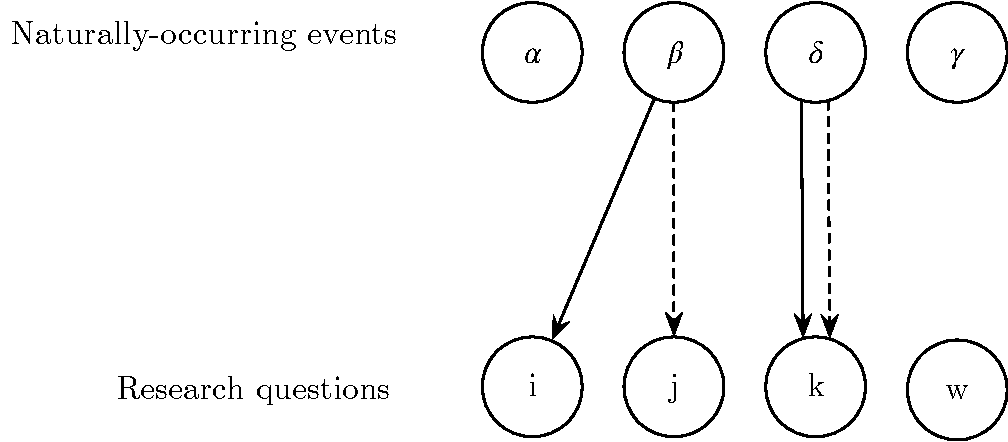
\includegraphics[width=0.7\textwidth]{exhibits/event_rq_mapping.pdf}
  \caption{Exogenous shocks map naturally-occurring events onto 
  research questions via empirical and substantive relevance. Notes.---
  
\includegraphics[width=0.075\textwidth]{exhibits/event_rq_mapping_0.pdf}
  = empirical relevance; 
  
\includegraphics[width=0.075\textwidth]{exhibits/event_rq_mapping_1.pdf}
   = substantive relevance.}
  \label{fig:event_rq_mapping}
\end{figure}

%% substantive relevance
The lack of \textit{substantive relevance} is one of the most common terrains 
where scholars have criticized the use of naturally-occurring events. For 
instance, in his critical analysis of Instrumental Variable (IV) applications,
\footnote{It is commonly accepted that natural experiments comprise the 
`Instrumental Variable' design along with the `Standard Natural Experiment' 
and `Regression Discontinuity Design' \autocite{sieweke_santoni_2020,dunning_2012}.} 
Deaton \autocite*{deaton_2009} observes that:

\begin{quote}
\textit{
  ``[omitted] randomized evaluations of projects are useful for obtaining a convincing
  estimate of the average effect of a program or project. The price for this
  success is a focus that is too narrow to tell us `what works' in development,
  to design policy, or to advance scientific knowledge about development
  processes.''
  }
  (page 3)
\end{quote}

Hence, he argues:

\begin{quote}
   \textit{
  ``[omitted] the analysis of programs or project needs to be refocused towards
  the investigation of potentially generalizable mechanisms that explain why and
  in what contexts projects can be expected to work. The best of the
  experimental work in development economics already does so, because its
  practitioners are too talented to be bound by their own methodological
  prescriptions. Yet there would be much to be said for doing so more openly. I
  concur with the general message in Pawson and Tilley (1997), who argue that
  thirty years of project evaluation in sociology, education and criminology was
  largely unsuccessful because it focused on whether projects work instead of on
  why they work.''
  }
  (page 4)
\end{quote}

Coming from an econometric background, Heckaman and Urzua
\autocite*{heckman_urzua_2010} share Deaton's concerns about IV as a lever to
approximate the experimental ideal:

\begin{quote}
  \textit{
  ``The problem that plagues the IV approach is that the questions it answers are
  usually defined as probability limits of estimators and not by well-formulated
  economic problems. Unspecified `effects' replace clearly defined economic
  parameters as the objects of empirical interest.''
  }
  (page 28)
\end{quote}

In his comprehensive work on natural experiments, Dunning 
\autocite*{dunning_2012} pragmatically points out:

\begin{quote}
  \textit{
  ``[omitted] the causes that Nature deigns to assign at random may not always be
  the most important causal variables for social scientists. For some observers,
  the proliferation of natural experiments therefore implies the narrowing of
  research agendas to focus on substantively uninteresting or theoretically
  irrelevant topics.''
  }
  (page 3)
\end{quote}

A positive example showing how to turn a naturally-occurring event into a shock
with substantive relevance is Miguel, Satyanath, and Sergenti's
\autocite*{miguel_et_al_2004} study of the effect of economic growth on civil
wars in Africa. Thanks to the ingenious choice to consider rainfall data,
the authors broaden the conversation on institutions and economic growth.
Particularly, rainfall variations facilitate an IV design that copes with
longstanding endogeneity issues regarding the co-evolution of institutions and
macroeconomic factors. Hence, the authors can empirically investigate a new
and essential theoretical relationship, namely, the effect of economic growth on
the likelihood of civil war. 

%% potential outcome framework
Regarding the \textit{empirical relevance} of a naturally-occurring event, the
literature on natural experiments shows a strict view: an event qualifies as an
exogenous shock if and only if it allows to operate an empirical strategy with
a control group \autocite[][]{cook_et_al_2002}. In other words, there should be
an adequate time window\footnote{We discuss the temporal aspects of exogeneous
shocks' effects in Section \ref{sec:how_exogenous_shocks_differ} and Section
\ref{sec:harnessing_exogenous_shocks}.} in which the intervention $T$ emerging
from the exogenous shock affects a fraction of a population's units only.  Such a
condition is the \textit{sine qua non} to evaluate the impact of the intervention
using Neyman's potential outcome framework \autocite*{neyman_et_al_1923}, an
unbiased estimator of the average causal effect $T - C$ that is based on three
quantities: (1) $\widehat{T}$, the average response if all subjects were assigned
to treatment; (2) $\widehat{C}$, the average response if all subjects were assigned
to control; and (3) the difference $\hat{T} - \widehat{C}$.

The study of John Snow of London's cholera outbreak of 1853-54\footnote{The
project of Snow --- aiming to prove that cholera did not transmit through the
air, the so called `miasma hypothesis'--- developed along two arms: he used
geospatial visualizations to show that attacks clustered around Broad Street
water pump in London's Soho district; then, he conducted the standard natural
experiment briefly summarized that we briefly summarize in the main text.}
emphasizes the importance of using exogenous shocks that heterogeneously affect
the units of a population. In 1852, the Lambeth Waterworks company --- one of
the major utility companies supplying water to several parts of the city ---
relocated their waterworks from Hungerford Market to fifteen miles upstream in
the Thames, thereby \textit{``obtaining a supply of water quite free from the
sewage of London''} \autocite[][page 68]{snow_1855}. Contrarily, Southwark \&
Vauxhall, a company competing with Lambeth Waterworks in several districts of
London, left its intake pipe downstream in the Thames at Battersea. Snow
obtained records on cholera deaths in households throughout London, as well as
information on the company that provided water to each household and the total
number of houses served by each company. Figure
\ref{fig:snow_natural_experiment} reports one of the most compelling pieces of
empirical evidence included the study: fatal attacks are compared before and
after the exogenous shock (Lambeth Waterworks moved their intake pipelines in
1952) and by water supply (see the column reported on the far-right hand section
of the table). Consistently with Neyman's model, the analyses of Snow disentangle
the `true' effect of the shock on cholera communication from time-invariant
attributes regarding the households served by different water suppliers, and,
perhaps more importantly, from the time-variant factors such as the state of the
cholera outbreak at other points in time. Should the naturally-occurring
event have affected the totality of households in London, unlikely Snow's work 
would have addressed the problem of confounders convincingly.  

\begin{figure}
  \begin{small}
    \begin{center}
      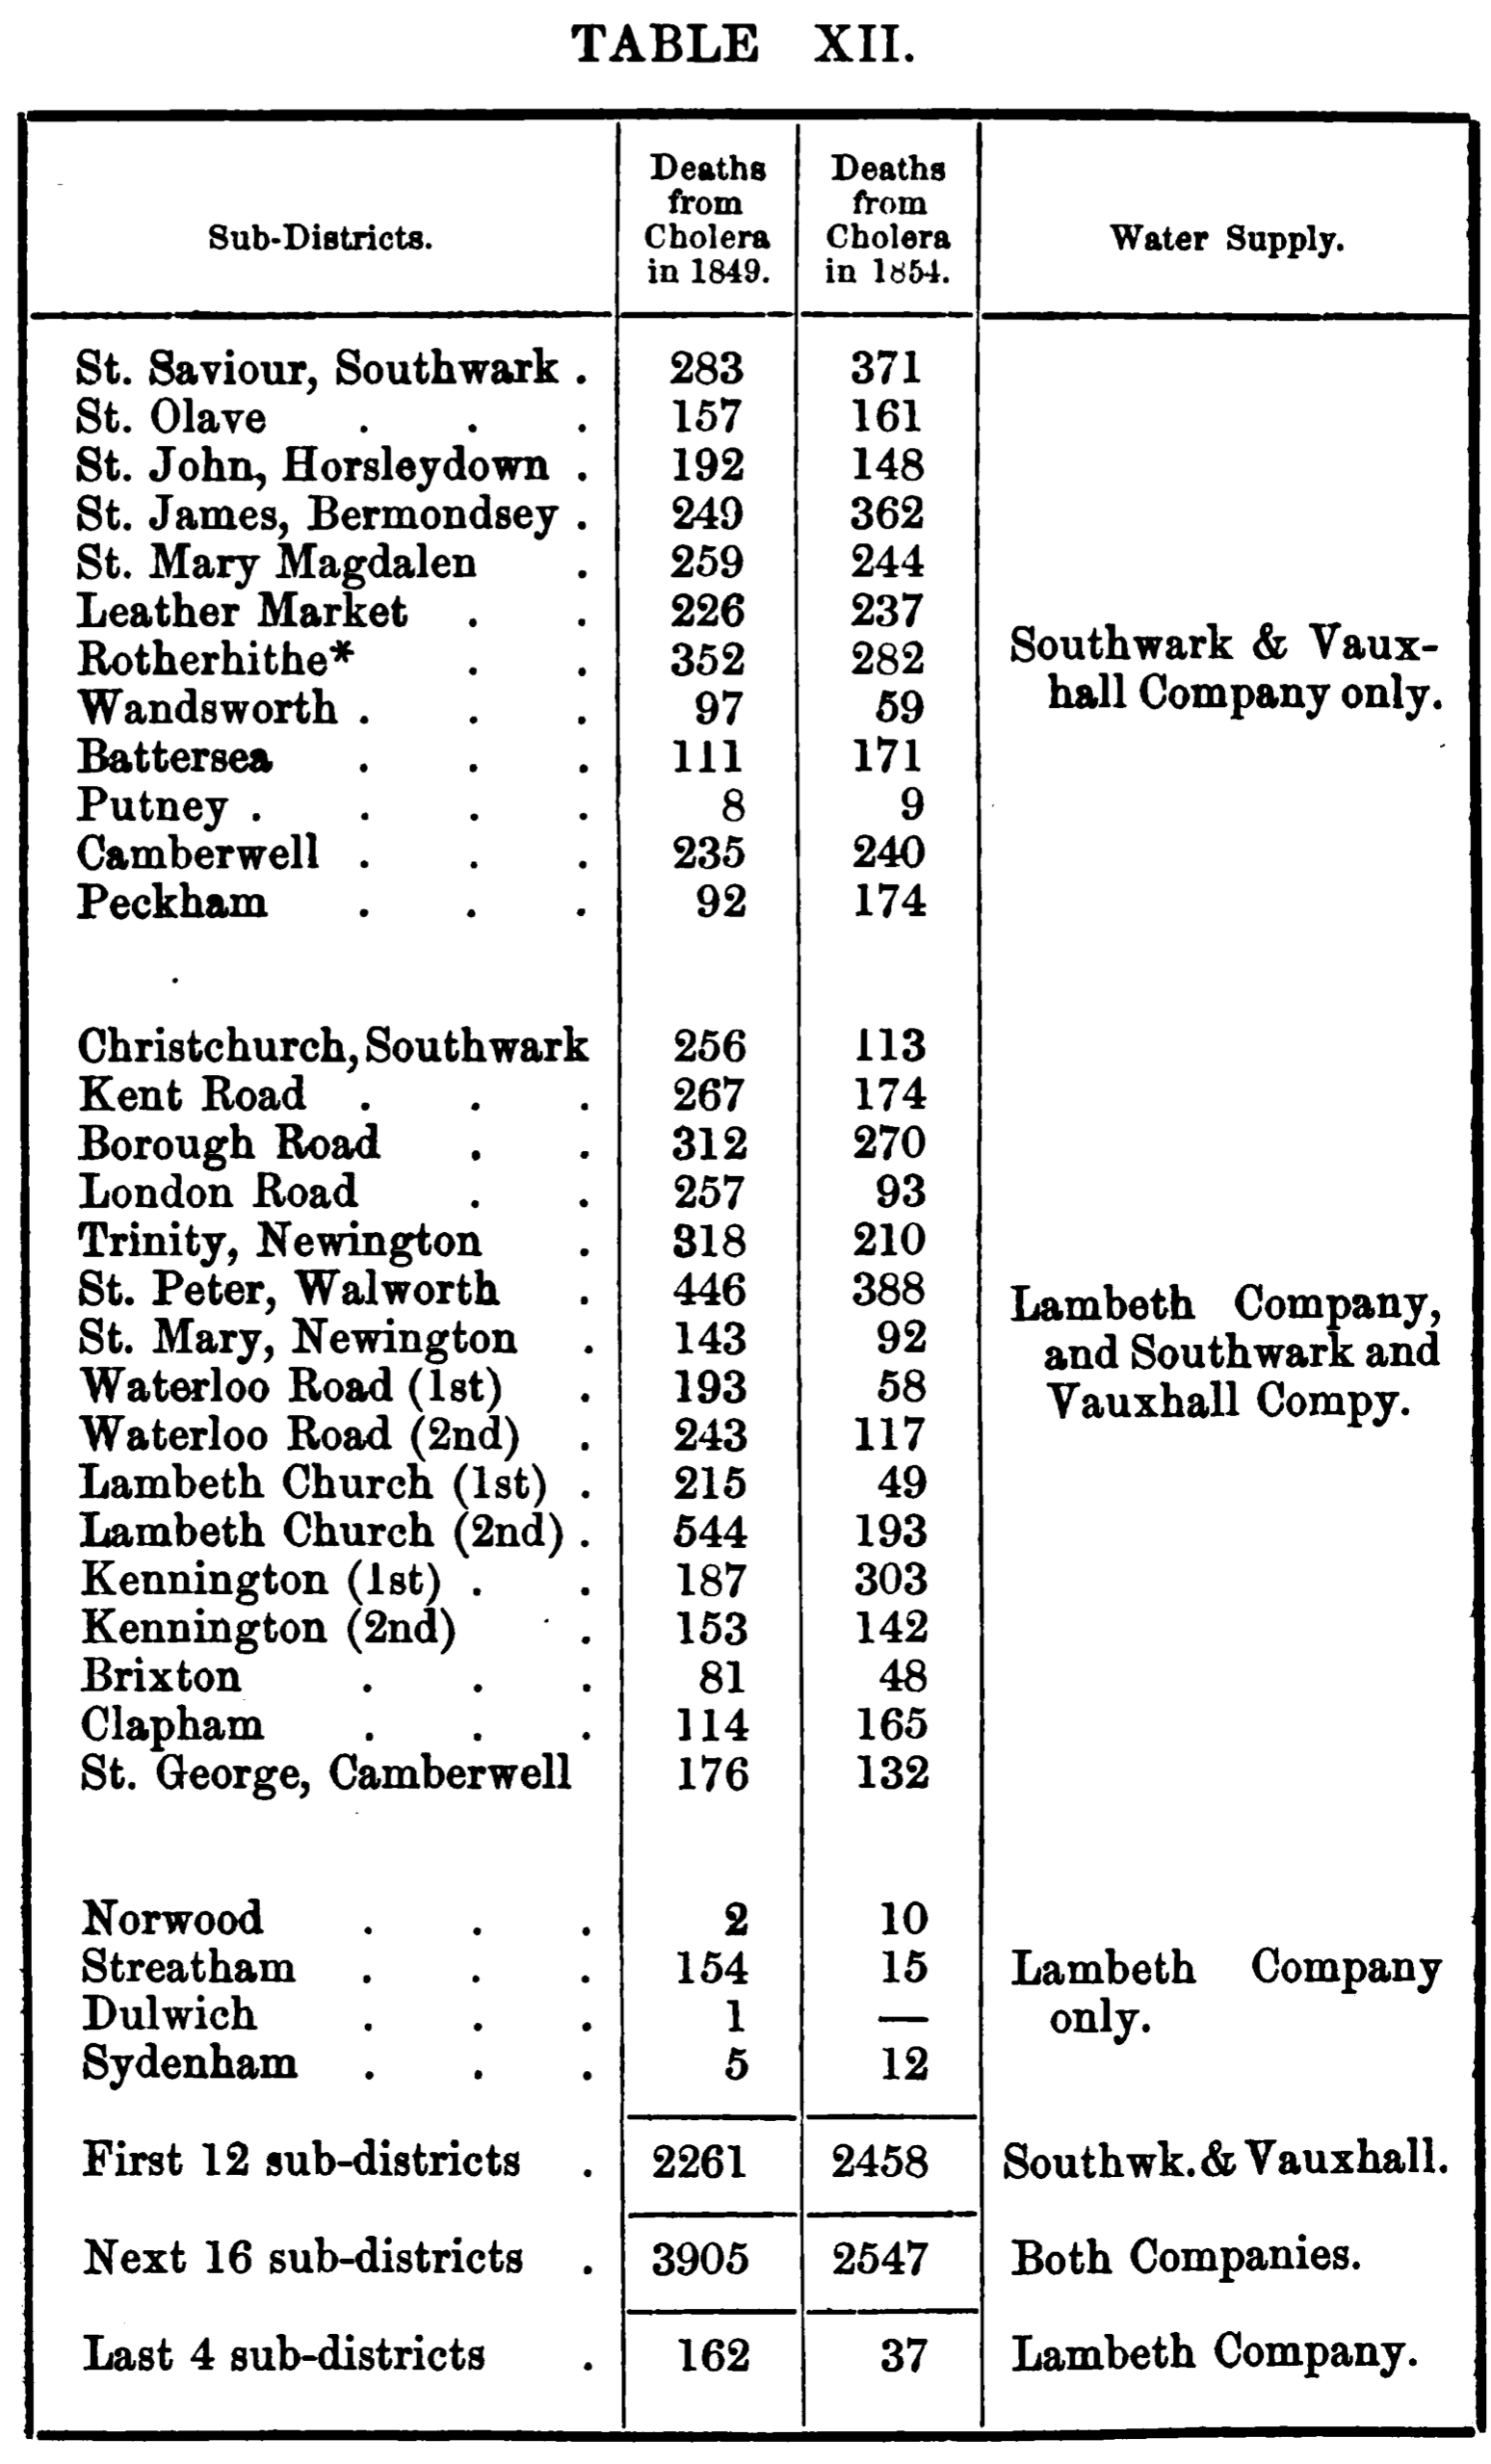
\includegraphics[width=0.8\textwidth]{exhibits/snow_natural_experiment.png}
    \end{center}
    \caption{An extract of the statistical analyses reported in the study of John 
    Snow `On the mode of communication of cholera' \autocite*{snow_1855}. The 
    table, reported on page 90, considers both pretest and posttest datapoints ---
    Lambeth Waterworks moved their intake pipes in 1952 --- for treated 
    and control households.}
    \label{fig:snow_natural_experiment}
  \end{small}
\end{figure}

%% sudden? out of control?
A related but distinct aspect of \textit{empirical relevance} concerns the
`exogenous' nature of the naturally-occurring variation. The literature on
natural experiments emphasizes that relevant events are not necessarily sudden,
such as the death of a business leader because of hearth attack
\autocite[e.g.,][]{nguyen_et_al_2010},\footnote{The identification of sudden
deaths poses definition issues
\autocite[e.g.,][]{azoulay_et_al_2010,oettl_2012}.  In the interest of
consistency, Nguyen and Nielsen \autocite*{nguyen_et_al_2010} report they
\textit{``rely on the medical literature, which defines sudden death as an
unexpected and non-traumatic death that occurs instantaneously or within a few
hours of an abrupt change in the person’s previous clinical state.''} The causes
of sudden deaths they consider are `hearth attack,' `stroke,' and `accident or
murder.' In addition to such deaths, they consider also \textit{``accidental 
and traumatic deaths that are unanticipated by the stock market and unrelated to
firm conditions''} (page 553). } uncontrollable, such as earthquakes
\autocite[e.g.,][]{belloc_et_al_2016}, or random, such as lotteries
\autocite[e.g.,][]{poulos_2019}.  Extant studies show that legal
changes and policy interventions can be purposefully used as exogenous shocks to
address particular research questions \autocites[e.g.,][]{beaman_et_al_2012,
matsa_miller_2013,chauchard_2014}. Dunning \autocite*[][page 236]{dunning_2012}
advances a three-step procedure to assess whether a naturally-occurring event
can be plausibly considered exogenous or `as-if random'. First, researchers
should investigate whether units had information that they would or would not
receive the treatment. Second, researchers need to check whether units had
incentives to self-select into the treatment group or control group. Third,
researchers should analyze whether not only units had incentives but also
capacity to self-select into a treatment status. For the assessment, Dunning
\autocite*{dunning_2012} suggests using both qualitative evidence (e.g.,
documents, interviews) and quantitative evidence (e.g., balance tests).

For example, Snow \autocite*{snow_1855} presented various sorts of evidence to
establish the pre-treatment equivalence of the houses that were exposed to pure
and contaminated sources of water supply:

\begin{quote}
  \textit{
  ``The mixing of the (water) supply is of the most intimate kind. The pipes of
  each Company go down all the streets, and into nearly all the courts and
  alleys. A few houses are supplied by one Company and a few by the other,
  according to the decision of the owner or occupier at that time when the Water
  Companies were in active competition. In many cases a single house has a
  supply different from that on either side. Each company supplies both rich and
  poor, both large houses and small; there is no difference either in the
  condition or occupation of the persons receiving the water of the different
  Companies\ldots It is obvious that no experiment could have been devised which
  would more thoroughly test the effect of water supply on the progress of
  cholera than this.''
  }
  \autocite[][pages 74 - 75]{snow_1855}
\end{quote}

At the same time, qualitative information on the context and the process that
determined the source of water-supply source was also essential for Snow.  For
instance, he emphasized that absentee landlords decided which competing water
companies would have served a particular address.  Thus, many residents had
limited opportunities to `self-select' into a source of water supply --- thus,
confounding characteristics of residents appeared unlikely to explain the large
differences in death rates by company (see Figure
\ref{fig:snow_natural_experiment}).  Moreover,  the Lambeth company committed to
moving their intake pipe upstream on the Thames before the cholera outbreak of
1853–54, when existing scientific knowledge did not link water sources to
cholera risk.  Such a supply choice implied that more than 300,000 people of 
all ages and social strata were

\begin{quote}
  \textit{``divided into two groups without their choice, and, in most cases, 
  without their knowledge; one group being supplied with water containing the 
  sewage of London, and, amongst it, whatever might have come from the cholera 
  patients, the other group having water quite free from such impurity.''}
  \autocite[][pages 74–75]{snow_1855}
\end{quote}

Drawing on the methodological insights included in Snow's study, Figure 
\ref{fig:exogeneous_shocks_and_ne} visually illustrates the idea that both
events that are unknown/unknowable to units and events that are known to units
can provide scholars with an exogenous variation suited to address the research 
question at hand.  However, `known events' may raise endogeneity concerns
regarding the possibility of a unit affecting the direction and magnitude of a
naturally-occurring variation and self-select into the treatment or control
group.

\begin{figure}[!htbp]
  %\sffamily
  \centering
  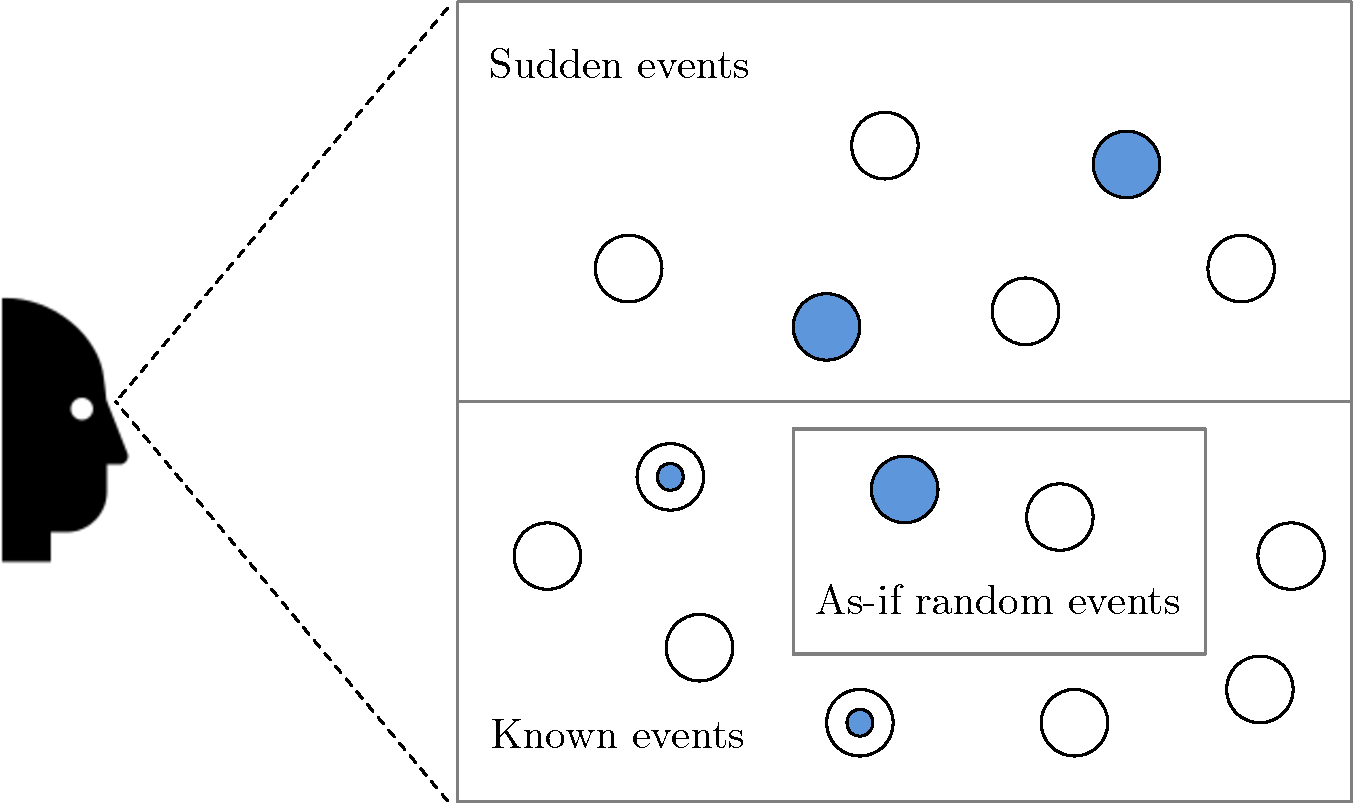
\includegraphics[width=1\textwidth]{exhibits/exogenous_shocks_and_ne.pdf}
  \caption{The interpretation of a naturally-occurring event as an exogenous 
  shock is contingent on the research question one wants to address and the 
  intrinsic attributes of the event. 
  Notes.---  
  
\includegraphics[width=0.02\textwidth]{exhibits/exogenous_shocks_and_ne_0.pdf}
  = exogenous shocks, i.e., naturally-occurring events that have empirical and/or 
  substantive relevance \textit{vis \'{a} vis} a target research question;
  
\includegraphics[width=0.0175\textwidth]{exhibits/exogenous_shocks_and_ne_2.pdf}
  = naturally-occurring events are not relevant to address a target research 
  question;
  
\includegraphics[width=0.0175\textwidth]{exhibits/exogenous_shocks_and_ne_1.pdf}
  = endogenous naturally-occurring events, i.e., environmental variations that 
  do not help to deal with the problem of confounders.}
  \label{fig:exogeneous_shocks_and_ne}
\end{figure}

\subsection{Exogenous shocks in leadership and management research}
\label{subsec:exogenous_shocks_in_management}

\noindent To understand how management scholars conceptualize and use
exogenous shocks, we conducted a systematic survey of the literature. 
Consistently with recently published reviews 
\autocite[e.g.,][]{gonzalez_et_al_2018,rindova_et_al_2018}, we restricted our
search to a selection of prominent journals such as Academy of Management
Journal, Administrative Science Quarterly, Entrepreneurship Theory and Practice,
Journal of Business Ethics, Journal of Business Venturing, Journal of
Management, Journal of Management Studies, The Leadership Quarterly, Management
Science, Organization Science, Organization Studies, Research Policy, Strategic
Entrepreneurship Journal, Strategic Management Journal, Strategic Organization.
Using Scopus, we retrieved articles published up until December 31, 2021
presenting the bi-gram `exogenous shock*,' in the title, abstract, \emph{or} set of
author's generated keywords. The search resulted in 49 unique items.
\footnote{Data were retrieved on January 17, 2022.}

Having considered the full manuscript of each retrieved articles, we discarded
18 articles that did not fall within the reviews's remit. Particularly, 
we excluded from the sample two studies in which the search token appears once and 
appears not to focus on or use the conceptual category of `exogenous shock'
\autocite{uzzi199735,kriauciunas2006659}; one work focusing on managers'
cognitive representation of a shock \autocite{barreto2013687}; four non-empirical papers
\autocite[e.g.,][]{mcsweeney2009933}; two qualitative studies
\autocite{glynn20051031, jenkins2010884}; one field experiment 
\autocite{cui20191216}; eight Management Science articles dealing with 
finance, marketing, or operations subjects \autocite[e.g.,][]{tham20182901}.
Figure~\ref{fig:studies_across_journals} illustrates the distribution of sample
studies across journals.

\begin{figure}[!htbp]
    \centering
    \import{}{exhibits/studies_across_journals.pgf}
    \caption{Distribution of studies that claim to use an exogenous shock across
    management journals.  Notes.--- N = 31; in the interest of consistency, we
    excluded `exogenous shock' studies published in Management Science addressing
    finance, marketing, or operations subjects. The following journals do not have any
    `exogenous shock' study: Administrative Science Quarterly, Entrepreneurship
    Theory and Practice, Journal of Business Venturing, Journal of Management,
    Leadership Quarterly, Research Policy.}
    \label{fig:studies_across_journals}
\end{figure}         

Two authors independently coded the retained studies against the dimensions 
included in Figure \ref{fig:event_rq_mapping}, that is, (1) the exploited 
naturally-occurring event (e.g., 9/11, Sarbane-Oxley Act); (2) the leading
research question (e.g., `how do changes in an employee's relational capital
influence mobility and entrepreneurship decisions?'); and (3) the relationship
between (1) and (2), which can be substantive --- when the exogenous shock is an
integral part of the research question/plays a key role for theorizing 
--- or empirical --- when one leverages an environmental variation to cope
with the problem of confounders, but the exogenous shock is unrelated with the
substantive scope of the study --- or both. Having completed the independent 
analysis of sample studies, the two authors merged their coding choices and 
reconciled their different views regarding the role of the exogenous shock 
in four papers.\footnote{The coding spreadsheet is publicly available at: \href{
  https://www.dropbox.com/s/yl0sf9p9tq253fy/coded_studies.csv?dl=0}
{https://www.dropbox.com/.../coded\_studies.xlsx?dl=0}.} 
Table \ref{tab:summary_of_studies} reports the outcome of our coding, including
a summary of how the naturally-occurring event qualifies as an exogenous
shock (see the column `Summary', reported on the right-hand side of the table).

Regarding the first dimension of our coding, the most popular categories of 
events are `legal change' and (N = 11) and `turnover' (N = 6) --- see Figure 
\ref{fig:classes_of_events}. Concerning `legal change,' scholars have relied on
events such as the staggered passage of anti-takeover laws 
\autocite{cabral202128,wang20162393}, change in immigration rules 
\autocite{choudhury2019203}, the Garn-St. Germain Act
\autocite{haveman2001253}, the Sarbane-Oxley Act \autocite{gupta2020802},
SEC's regulation change \autocite{jia2020290}, the change of inheritance, gift,
and estate taxes \autocite{kang20201300}, the staggered adoption of the
Inevitable Disclosure Doctrine in U.S. \autocite{kang20201300}, a revision of
U.S. Higher Education Amendments \autocite{krishnan20194522}, reductions in
import tariffs \autocite{li20194011}, demonetization measures
\autocite{natarajan20191070}.  Turnover events comprise sick leave episodes of
key employees \autocite{chen20181239,drexler20142722,chown2015177,}, political
leadership churn \autocite{birhanu2020,byun20191368}, and sudden deaths
of executives \autocite{ke2019439}. Other recurrent events include terrorist
attacks \autocite{corbo2016323,vergne20121027,li20194011} and scandals
\autocite{cai2019159,hilary2021}, and change in financial analysts' coverage
\autocite{chatterji2010917,qian20192271}.

\begin{figure}[!htbp]
    \centering
    \import{}{exhibits/classes_of_events.pgf}
    \caption{Classes of naturally-occurring events presumed to create 
    exogenous shocks.}
    \label{fig:classes_of_events}
\end{figure}

As shown in the Venn diagram included in Figure \ref{fig:event_roles}, the large
majority of the cases included in our sample (N = 24) claim to use exogenous
shocks with an empirical role. For instance, Krishnan and Wang
\autocite*{krishnan20194522} use Survey of Consumer Finances data to address the
research question `does student debt influence the propensity to start a firm?'.
The concept of exogenous shock is not important for the scope of their work and
does not inform the proposed theorizing. At the same time, one may study the
relationship between student debt and business creation in the context of an
observational empirical strategy. However, the authors are concerned about the
causal interpretation of their empirical estimates:

\begin{quote}
  \textit{
  ``there may be unobserved characteristics that may drive our results. For
  instance, individuals with wealthier families may have lower student debt as
  well as the financial means to start a firm. Such unobservable family effects
  may explain the negative relation between student debt and entrepreneurship.
  Alternatively, individuals from wealthier families may borrow more if they
  expect to be able to pay back the loans easily (and such individuals are more
  likely to be entrepreneurs).''
  }
  (page 4528)
\end{quote}

\begin{figure}[!htbp]
    \centering
    \import{}{exhibits/event_roles.pgf}
    \caption{Role of the naturally-occurring events presumed to create exogenous shocks.}
    \label{fig:event_roles}
\end{figure}

Hence, they use a legal change as an exogenous shock to the cost of business 
failures for individuals with greater levels of student loans:

\begin{quote}
  \textit{
  ``To address endogeneity concerns, we utilize the Higher Education Amendments
  (HEA) of 1998, which effectively rendered student loans completely
  non-dischargeable. We find that students that were already in four-year college
  at the time of this regulation and had significant student debt were less
  likely to start a firm. This test considers only individuals who were enrolled
  prior to the year of regulation (i.e., prior to 1998) in a four-year college.
  The idea is that, for the group of individuals who are already enrolled in
  college, the regulatory change is clearly exogenous, in the sense that it
  does not drive their choice to enter college. ''
  }
  (page 4532)
\end{quote}

Half of the studies circa (N = 15) assign a substantive role to exogenous
shocks.  For example, Haveman, Russo and Meyer \autocite*{haveman2001253} 
articulate a framework that links organizations' responses to discontinuous
industry-level regulatory change. The theoretical section of the study maps the
phenomenon of regulatory change onto the General Punctuated Equilibrium Model
and provides expectations about the multiple consequences of regulatory change
for individual organizations. The substantive role of the shock is self-evident
in the formulation of the hypotheses, e.g.:

\begin{quote}
  \textit{
    ``Immediately following any regulatory punctuation, CEO succession rates
    will not rise; instead, CEO succession rates will rise gradually as time
    passes.''
  }
  (page 259)
\end{quote}

It is worth notice the authors emphasize the `exogenous' nature of the Garn-St.
Germain Act --- the example of regulatory change at the center of the paper 
---, but they do not discuss what it means for the empirical strategy of 
the study, and, especially, in terms of empirical identification.

We also found a subset of studies (N = 8) that claim to use an exogenous with
empirical and substantive relevance. Byun, Raffaele, and Ganco
\autocite{byun20191368} propose a hypothesis set that connect `discontinuous
increases in the value of an employee's relational capital' with `employee
turnover' and `spinout' formation. For example, their first hypothesis states:

\begin{quote}
  \textit{
    ``Discontinuous increases in the value of an  employee's relational capital 
    will be positively related to employee exit.''
  }
  (page 1371)
\end{quote}

The authors can advance and test this and the other hypotheses thanks to
naturally-occuring events regarding the politicians connected to lobbyists
(i.e., `employees').  Here is a passage concerning the description of the
independent variable of the study, `discontinuous increases in the value of an
employee's relational capital:'

\begin{quote}
  \textit{
    ``We use appointments to committee chair and assignments to the four most
    powerful committees in Congress to capture connected politicians' power
    changes in the legislative process. Discontinuous increase is a binary
    variable coded `1' for the first year a politician connected to a lobbyist is
    selected to be a chair of a congressional committee or is assigned to one of
    the powerful committees in Congress and `0' otherwise.''
  }
  (page 1375)
\end{quote}

The series of political appointment decisions also play an empirical role, the 
Byun and colleagues point out: 

\begin{quote}
  \textit{
    ``Our identifying assumption is consistent with prior work and rests on the
    notion that the temporal change in power of connected politicians is
    exogenous, conditional on the observable characteristics of the lobbyists
    and their firms [omitted]. For the power change of a connected politician to
    be plausibly exogenous, whether and when the connected politician will
    experience the advancement has to be difficult to predict by lobbyists and
    firms. In addition, the change in lobbyist's value creation due to a surge
    in the value of political connections should be uncorrelated with the
    accumulation of the lobbyist's expertise, conditional on observables. Given
    the complicated and uncertain political process of chair selection and
    committee assignment, scholars have argued that committee and chair
    assignment satisfies these conditions with respect to lobbyists [omitted].
    In fact, others have gone as far as to argue that the timing and ascension
    of committee and chair appointments are exogenous even to the politician
    herself [omitted]. Thus, it is reasonable to believe that using the power
    change of a connected politician to capture discontinuous in-creases in the
    lobbyist's relational capital would alleviate identification concerns due to
    potential omitted variable biases.''
  }
  (page 1375)
\end{quote}

\begin{figure}
  \raggedleft
  \begin{small}
    \import{}{exhibits/potential_outcome.pgf}
    \caption{
      Distribution of studies across empirical strategies and exogenous shocks'
      roles. Notes. --- A design lacking a control group has pretest and posttest
      observations for one group only; a design with a control group has
      pre-test and post-test both for units that are affected by the exogenous
      shock and those that are not.
    }
    \label{fig:potential_outcome}
  \end{small}
\end{figure}

Figure \ref{fig:potential_outcome} illustrates the distribution of sample
studies across empirical strategies and exogenous shocks' roles. Circa one-third of 
the articles (N = 11) operate an empirical strategy without a control group. Within 
this group, we found three articles that do not use the shock for empirical 
identification purposes. For example, Corbo, Ferriani, and Corrado
\autocite*{corbo2016323} use 9/11 as a \textit{``major environmental shock''}
(page 323), affecting the logic that shapes the formation of alliances in the
airline industry. The impact of 9/11 on aviation companies is so sudden and
pervasive to impede the identification of units that can form a control group
even for a limited amount of time.  Although such a naturally-occurring
variation does not facilitate empirical identification, it is relevant from a
substantive standpoint. According to the authors, 9/11 allows them to explore
novel theoretical intuitions regarding the change of interorganizational
networks:

\begin{quote}
  \textit{
    ``Our intuition is that patterns of interorganizational network ties provide
    a lens through which to view critical junctures that question extant logics
    and open prospects for change, enabling us to shed light on organizational
    responses to external events.  To explore these ideas empirically and inform
    our understanding of the interorganizational dynamics characterizing fields
    that undergo cataclysmic upheavals, we focus on the global airline industry
    in the aftermath of the September 11, 2001 terrorist attacks (henceforth
    9/11), which caused one of the most severe crises ever experienced by civil
    aviation worldwide. Given the exploratory, theory-building nature of the
    study we employ a hybrid empirical strategy that combines qualitative data
    analysis with quantitative social network analysis, enabling us to capture a
    more complete, holistic and contextual portrayal of the units under study
    [omitted].''
  }
  (page 325)
\end{quote}

The remaining eight articles lacking a control group emphasize the empirical
relevance of their naturally-occurring events. Seebeck and Vetter
\autocite*{seebeck2021} investigate the relationship between gender board
diversity and corporate risk disclosure.  The study uses the Brexit Referendum
to create an intention-to-treat model where the future exit of the United
Kingdom from the European Union is an exogenous shock on firm's risk environment
by which:

\begin{quote}
  \textit{
    ``all firms face similar and tremendous risks related to the Brexit that
    need to be considered by public firms when preparing their annual reports
    according to the Financial Reporting Council (FRC 2016a, b) as well as
    section 414c(2)(b) of the companies act and section 4 of the UK corporate
    governance code.''
  }
\end{quote}

The authors claim to advance the literature on gender diversity and 
corporate governance by dealing with the endogeneity of a firm's risk 
reporting needs. Specifically, they assert their empirical strategy

\begin{quote}
  \textit{
    ``is less likely to face the risk of omitted variables, allowing to
    provide more reliable evidence of an association between board gender diversity
    and corporate risk disclosure.''
  }
\end{quote}

However, Seebeck and Vetter's article does not implement Neyman Potential Outcome
Framework because the study sample includes UK (FTSE 350) companies only, 
affected by the exogenous shock.

% define new column type
\newcolumntype{Y}[1]{%
  >{\small\raggedright\everypar{\hangindent=1em}\arraybackslash}p{#1}%
}
% define newline to use hangindent on new line
\renewcommand{\arraystretch}{1.3}

\begin{sidewaystable}[!htbp]
  \centering
  %\sffamily
  \begin{small}
    \caption{\textsc{Summary of study events, research questions, and 
    exogenous shocks}}
    \vspace{-1.75em}
    \label{tab:summary_of_studies}
    \begin{center}
       %\resizebox{1\textwidth}{!}{%
       \begin{tabular}{{@{\extracolsep{2pt}} 
         p{3.85cm}@{\hskip 4mm}   %1 
         Y{4cm}@{\hskip 4mm}   %2
         Y{4cm}@{\hskip 4mm}   %3
         p{0.5cm}@{\hskip 4mm}   %4
         p{0.5cm}@{\hskip 4mm}   %5
         Y{7cm}@{\hskip 4mm} %6
         }}
         \toprule \toprule
         & %1
         & %2
         & %3
         \multicolumn{3}{l}{Relevance of the event}\\ \cmidrule{4-6}
         \multicolumn{1}{l}{Study} &
         \multicolumn{1}{l}{Event} &
         \multicolumn{1}{l}{Research question} &
         \multicolumn{1}{c}{Empirical} &
         \multicolumn{1}{c}{Substantive} &
         \multicolumn{1}{l}{Summary}\\
         \midrule \\[-1.8ex]

         Birhanu \& Wezel \autocite*{birhanu2020}\dotfill &
         Government changes following Arab spring social movement. &
         How does group affiliation influence firm performance under weak market
         institutions?&
         \multicolumn{1}{c}{$\checkmark$} &
         \multicolumn{1}{c}{$\times$} &
         The use of sudden government change is presumed to affect executives'
         capacity to influence political leaders.\\ \\[-1.8ex]

         Byun et al. \autocite*{byun20191368}\dotfill&
         Change in a politician's committee and/or committee chair assignments. &
         How do changes in an employee's relational capital influence mobility 
         and entrepreneurship decisions? &
         \multicolumn{1}{c}{$\checkmark$} &
         \multicolumn{1}{c}{$\checkmark$} &
         Lobbyists may experience a discontinuous shift in the value associated
         with a connection if there are changes to a politician's committee
         and/or committee chair assignments. Then, the authors can
         investigate empirically the consequences of social capital change on
         lobbyists' career. \\ \\[-1.8ex]
         
         Cabral et al. \autocite*{cabral202128}\dotfill&
         Staggered passage of anti-takeover laws in U.S. &
         Does managerial job security affect the adoption of innovative 
         practices and structures?&
         \multicolumn{1}{c}{$\checkmark$} &
         \multicolumn{1}{c}{$\checkmark$} &
         The adoption of an anti-takeover statute is a proxy of managerial job
         security, which changes across states and within individual states over
         time, and is supposed to affect the propensity to create a CVC
         program. \\ \\[-1.8ex]

         Cai \& Shi \autocite*{cai2019159}\dotfill &
         Revelation of the sex abuse of children by Catholic priests in U.S. &
         Does a firm's religious environment influence outside parties' 
         perceptions in contracting with the firm? &
         \multicolumn{1}{c}{$\checkmark$} &
         \multicolumn{1}{c}{$\times$} &
         Revelation of the sex abuse of children by Catholic priests is an
         exogenous shock to the religiosity of a region, which  can 
         influence the capital structure, credit rating, cost of debt, and
         covenants of local firms.\\ \\[-1.8ex]
         \bottomrule
       
        \end{tabular}
       %} 
    \end{center}
  \end{small}
\end{sidewaystable}

\begin{sidewaystable}[!htbp]
  \centering
  %\sffamily
  \begin{small}
    \caption*{\textsc{Table I} (\textsc{cont'd})}
    \vspace{-1.75em}
    \begin{center}
       %\resizebox{1\textwidth}{!}{%
       \begin{tabular}{{@{\extracolsep{2pt}}
         p{4.20cm}@{\hskip 4mm}   %1 
         Y{4cm}@{\hskip 4mm}   %2
         Y{4cm}@{\hskip 4mm}   %3
         p{0.5cm}@{\hskip 4mm}   %4
         p{0.5cm}@{\hskip 4mm}   %5
         Y{7cm}@{\hskip 4mm} %6
         }}
         \toprule \toprule
         & %1
         & %2
         & %3
         \multicolumn{3}{l}{Relevance of the event}\\ \cmidrule{4-6}
         \multicolumn{1}{l}{Study} &
         \multicolumn{1}{l}{Event} &
         \multicolumn{1}{l}{Research question} &
         \multicolumn{1}{c}{Empirical} &
         \multicolumn{1}{c}{Substantive} &
         \multicolumn{1}{l}{Summary}\\
         \midrule \\[-1.8ex]

         Chatterji \& Fabrizio \autocite*{chatterji2016447}\dotfill&
         Department of Justice investigation against the five largest U.S. 
         orthopedic device makers.&
         How does an open system of innovation affect the rate and direction 
         of innovation?&
         \multicolumn{1}{c}{$\checkmark$} &
         \multicolumn{1}{c}{$\times$} &       
         Department of Justice investigation increases the frictions in the 
         market for ideas by regulating the interactions between physicians 
         and the medical device firms under investigation.\\
         \\[-1.8ex]
         
         Chatterji \& Toffel \autocite*{chatterji2010917}\dotfill&
         Change in the scope of KLD Database, a prominent source of CSR ratings.&
         How do managers react to poor corporate environmental ratings?&
         \multicolumn{1}{c}{$\checkmark$} &
         \multicolumn{1}{c}{$\checkmark$} &       
         The change in KLD's scope creates a subset of
         companies responding for the first time to a CSR rating, which allows
         the authors to deal with mutual causality issues regarding a firm's CSR
         rating and CSR strategy.\\ \\[-1.8ex]
         
         Chen \& Garg \autocite*{chen20181239}\dotfill &
         Injuries occurring to star NBA players. &
         Does a star's temporary absence help the organization overcome myopia?&
         \multicolumn{1}{c}{$\checkmark$} &
         \multicolumn{1}{c}{$\checkmark$} &       
         The absence of star players is presumed to impact the pattern of
         organizational routines at the team level. \\ \\[-1.8ex]
         
         Choudhury \& Kim \autocite*{choudhury2019203}\dotfill&
         Change in U.S. H1B employment visas.&
         How do migrant inventors influence knowledge production and reuse? &
         \multicolumn{1}{c}{$\checkmark$} &
         \multicolumn{1}{c}{$\times$} &
         The H1B quota change exempted universities and a selected list of other
         entities, creating heterogeneous effects in terms of supply of first-generation
         ethnic migrant inventors and the rate of codification of knowledge
         previously locked within migrant inventors' home countries.\\ \\[-1.8ex]

         \bottomrule
        \end{tabular}
        %} 
      \end{center}
    \end{small}
  \end{sidewaystable}
  
\begin{sidewaystable}[!htbp]
    \centering
    %\sffamily
    \begin{small}
      \caption*{\textsc{Table I} (\textsc{cont'd})}
      \vspace{-1.75em}
      \begin{center}
        %\resizebox{1\textwidth}{!}{%
        \begin{tabular}{{@{\extracolsep{2pt}}
          p{3.85cm}@{\hskip 4mm}   %1 
          Y{4cm}@{\hskip 4mm}   %2
          Y{4cm}@{\hskip 4mm}   %3
          p{0.5cm}@{\hskip 4mm}   %4
          p{0.5cm}@{\hskip 4mm}   %5
          Y{7cm}@{\hskip 4mm} %6
          }}
          \toprule \toprule
          & %1
          & %2
          & %3
          \multicolumn{3}{l}{Relevance of the event}\\ \cmidrule{4-6}
          \multicolumn{1}{l}{Study} &
          \multicolumn{1}{l}{Event} &
          \multicolumn{1}{l}{Research question} &
          \multicolumn{1}{c}{Empirical} &
          \multicolumn{1}{c}{Substantive} &
          \multicolumn{1}{l}{Summary}\\
          \midrule \\[-1.8ex]

         Chown \& Liu \autocite*{chown2015177}\dotfill &
         Turnover within U.S. Senate and `iconoclastic' senators deviating from 
         the institutionalized seating arrangement. &
         How does one's location in an organizational forum affect the
         likelihood to receive support from peers?&
         \multicolumn{1}{c}{$\checkmark$} &
         \multicolumn{1}{c}{$\times$} &
         Turnover within U.S. Senate and `iconoclastic' senior senators create
         opportunities for freshman senators not to seat at the margins of the
         chamber. These elements affect the dyadic distance between senators, a factor
         that is presumed to affect the likelihood of joint support. \\ \\[-1.8ex]

         Corbo et al. \autocite*{corbo2016323}\dotfill&
         9/11.&
         Does a major environmental shock affect the social structure of an 
         organizational field?&
         \multicolumn{1}{c}{$\times$} &
         \multicolumn{1}{c}{$\checkmark$} &
         9/11 is supposed to affect the organization and functioning of civil
         aviation, which allows the authors to assess the extent with which
         network mechanisms shape the alliances connecting airline companies 
         under different contingencies.\\ \\[-1.8ex]

         Drexler \& Schoar \autocite*{drexler20142722}\dotfill &
         Sick leave episodes among loan officers &
         How (much) does employee turnover affect organizational performance? &
         \multicolumn{1}{c}{$\checkmark$} &
         \multicolumn{1}{c}{$\checkmark$} &
         Loan officers' sick leaves alter economic and social exchange between
         the firm and its clients.\\ \\[-1.8ex]
        
         Gupta et al. \autocite*{gupta2020802}\dotfill &
         Sarbanes-Oxley Act (SOX) \& Global Financial Crisis &
         Does CFO gender influence the likelihood of financial misreporting? &
         \multicolumn{1}{c}{$\checkmark$} &
         \multicolumn{1}{c}{$\times$} &
         The authors expect: i) SOX to lead to a larger decrease in financial
         misreporting for male CFO firms than female-CFO firm; ii) firms to face
         greater pressure to report favorable earnings during crisis periods,
         which is more likely to influence male compared to female CFOs (based
         on the logic that female CFOs will be less likely to engage in fraud
         regardless of stakeholder pressure).\\  \\[-1.8ex]
          
         \bottomrule
       \end{tabular}
       %} 
    \end{center}
  \end{small}
\end{sidewaystable}

\begin{sidewaystable}[!htbp]
  \centering
  %\sffamily
  \begin{small}
    \caption*{\textsc{Table I} (\textsc{cont'd})}
    \vspace{-1.75em}
    \begin{center}
       %\resizebox{1\textwidth}{!}{%
       \begin{tabular}{{@{\extracolsep{2pt}}
         p{3.85cm}@{\hskip 4mm}   %1 
         Y{4cm}@{\hskip 4mm}   %2
         Y{4cm}@{\hskip 4mm}   %3
         p{0.5cm}@{\hskip 4mm}   %4
         p{0.5cm}@{\hskip 4mm}   %5
         Y{7cm}@{\hskip 4mm} %6
         }}
         \toprule \toprule
         & %1
         & %2
         & %3
         \multicolumn{3}{l}{Relevance of the event}\\ \cmidrule{4-6}
         \multicolumn{1}{l}{Study} &
         \multicolumn{1}{l}{Event} &
         \multicolumn{1}{l}{Research question} &
         \multicolumn{1}{c}{Empirical} &
         \multicolumn{1}{c}{Substantive} &
         \multicolumn{1}{l}{Summary}\\
         \midrule \\[-1.8ex]

         Haveman et al. \autocite*{byun20191368}\dotfill&
         California Legislature enactment of the nation's first comprehensive 
         managed competition program, and Garn-St. Germain Act&
         How do organizations respond to discontinuous indsutry-level change?&
         \multicolumn{1}{c}{$\times$} & 
         \multicolumn{1}{c}{$\checkmark$} &
         The authors use a series of regulatory changes to investigate how
         organizations respond to punctuated changes in the environment and with
         what performance consequences.\\ \\[-1.8ex]
          
         Hilary \& Huang \autocite*{hilary2021}\dotfill &
         Revelation of the sex abuse of children by Catholic priests in U.S. &
         Does generalized trust affect the power of CEO contracts? & 
         \multicolumn{1}{c}{$\checkmark$} & 
         \multicolumn{1}{c}{$\times$} &
         Revelation of the sex abuse of children by Catholic priests
         reduces generalized trust for certain counties only, which helps to reveal
         the causal effect of generalized trust on the characteristics of
         executives' contracts.\\ \\[1.8ex] 

         Jia et al. \autocite*{jia2020290}\dotfill&
         2005 Regulation SHO by which SEC removes the uptick restriction for a
         set of randomly selected pilot firms.&
         Do managers use CSR to insure against stock price risk?&
         \multicolumn{1}{c}{$\checkmark$} & 
         \multicolumn{1}{c}{$\times$} &
         SEC program changes stock risk price for pilot firms only, which helps
         to assess whether firms invest in CSR in response to greater stock
         price risk, and whether such investments provide intended
         insurance-like benefits.\\ \\[-1.8ex]

         Kang \& Kim \autocite*{kang20201300}\dotfill &
         Staggered changes in inheritance, gift, and estate 
         taxes in U.S. \& sudden deaths of business owners. &
         Do family-firms invest more in employee relations than 
         non-family firms? & 
         \multicolumn{1}{c}{$\checkmark$} & 
         \multicolumn{1}{c}{$\times$} &
         Taxation changes provide family owners with
         incentives to continue their businesses, which helps to
         reveal the relationship between governance forms and investment in
         employee relations.

         Sudden death of family members alter a firm's status, which 
         attenuates the concerns time-invariant characteristics jointly 
         affect performance and ability to implement employee-friendly 
         policies.\\ \\[-1.8ex]

         \bottomrule
       \end{tabular}
       %} 
    \end{center}
  \end{small}
\end{sidewaystable}

\begin{sidewaystable}[!htbp]
  \centering
  %\sffamily
  \begin{small}
    \caption*{\textsc{Table I} (\textsc{cont'd})}
    \vspace{-1.75em}
    \begin{center}
       %\resizebox{1\textwidth}{!}{%
       \begin{tabular}{{@{\extracolsep{2pt}}
         p{3.85cm}@{\hskip 4mm}   %1 
         Y{4cm}@{\hskip 4mm}   %2
         Y{4cm}@{\hskip 4mm}   %3
         p{0.5cm}@{\hskip 4mm}   %4
         p{0.5cm}@{\hskip 4mm}   %5
         Y{7cm}@{\hskip 4mm} %6
         }}
         \toprule \toprule
         & %1
         & %2
         & %3
         \multicolumn{3}{l}{Relevance of the event}\\ \cmidrule{4-6}
         \multicolumn{1}{l}{Study} &
         \multicolumn{1}{l}{Event} &
         \multicolumn{1}{l}{Research question} &
         \multicolumn{1}{c}{Empirical} &
         \multicolumn{1}{c}{Substantive} &
         \multicolumn{1}{l}{Summary}\\
         \midrule \\[-1.8ex]

         Ke et al. \autocite*{ke2019439}\dotfill &
         Sudden deaths and retirements of executives. &
         How do social connections among executive team members affect 
         management forecast accuracy?&
         \multicolumn{1}{c}{$\checkmark$} & 
         \multicolumn{1}{c}{$\times$} &
         Sudden turnover events alter the social connections within a team of
         executives, and, in turn, help to reveal the causal effect of social
         capital on decision-making quality. \\ \\[-1.8ex]
         
         Koh et al. \autocite*{koh20185725}\dotfill &
         Staggered adoption of the Inevitable Disclosure Doctrine (IDD).
         in U.S. &
         Are confident CEOs more likely to report R\&D expenditures than
         cautious CEOs? &
         \multicolumn{1}{c}{$\checkmark$} & 
         \multicolumn{1}{c}{$\times$} &
         The staggered U.S. state courts' verdict on the IDD helps to
         reveal the relationship between CEO confidence and R\&D disclosure by
         attenuating market competition.\\ \\[-1.8ex] 

         Krishnan \& Wang \autocite*{krishnan20194522}\dotfill&
         1992 and 1998 Higher Education Amendments (HEA) &
         How does student debt influence the propensity to start a firm? &
         \multicolumn{1}{c}{$\checkmark$} & 
         \multicolumn{1}{c}{$\times$} &
         1998 HEA alters the cost of discharging student debt through bankruptcy
         --- which increases the cost of entrepreneurship, that is, new venture
         failure --- while it is unlikely to affect financing availability to start
         a venture. Hence, the authors can assess the causal relationship
         linking student debt with propensity to create a new venture.
         
         1992 HEA affects the volume of student loans thought the federal
         government.  Students who spend more time in college during the
         post-1992 HEA regime will have more student loans. Hence, they will
         have lower likelihood to start a new venture. \\ \\[-1.8ex]

         Li \& Tallman \autocite*{li20111119}\dotfill&
         9/11.&
         Does a sudden change in the environment influence the economic 
         returns of international diversification?&
         \multicolumn{1}{c}{$\times$} & 
         \multicolumn{1}{c}{$\checkmark$} &
         9/11 is a ``reorienting disruptive change'' that alters international
         business logics, particularly, the economic and finial returns of
         international diversification.\\ \\[-1.8ex]
         
         \bottomrule
       \end{tabular}
       %} 
    \end{center}
  \end{small}
\end{sidewaystable}

\begin{sidewaystable}[!htbp]
  \centering
  %\sffamily
  \begin{small}
    \caption*{\textsc{Table I} (\textsc{cont'd})}
    \vspace{-1.75em}
    \begin{center}
       %\resizebox{1\textwidth}{!}{%
       \begin{tabular}{{@{\extracolsep{2pt}}
         p{3.85cm}@{\hskip 4mm}   %1 
         Y{4cm}@{\hskip 4mm}   %2
         Y{4cm}@{\hskip 4mm}   %3
         p{0.5cm}@{\hskip 4mm}   %4
         p{0.5cm}@{\hskip 4mm}   %5
         Y{7cm}@{\hskip 4mm} %6
         }}
         \toprule \toprule
         & %1
         & %2
         & %3
         \multicolumn{3}{l}{Relevance of the event}\\ \cmidrule{4-6}
         \multicolumn{1}{l}{Study} &
         \multicolumn{1}{l}{Event} &
         \multicolumn{1}{l}{Research question} &
         \multicolumn{1}{c}{Empirical} &
         \multicolumn{1}{c}{Substantive} &
         \multicolumn{1}{l}{Summary}\\
         \midrule \\[-1.8ex]

         Li \& Zhan \autocite*{li20194011}\dotfill&
         Reductions in import tariffs initiated by U.S. authorities. &
         How does product market threats affect stock crash risk?&
         \multicolumn{1}{c}{$\checkmark$} & 
         \multicolumn{1}{c}{$\times$} &
         Reduction in import tariffs increases competitive pressure, which 
         aggravates executives' incentive to withhold negative information 
         and increases and make firms more prone to stock crashes.\\ \\[-1.8ex]

         Mahmood et al. \autocite*{mahmood20171082} \dotfill &
         Global Financial Crisis.&
         How does centralization of intragroup equity ties affects the 
         performance of group affiliates?&
         \multicolumn{1}{c}{$\checkmark$} & 
         \multicolumn{1}{c}{$\checkmark$} &
         Global Financial Crisis creates environmental turbulence exogenously
         for Taiwanese firms, and, in turn, helps to appreciate the
         contingent role of equity tie centralization.\\ \\[-1.8ex]

         Natarjan et al. \autocite*{natarajan20191070}\dotfill&
         Indian Government's demonetization measure.&
         How do middle managers influence resource allocation choices?&
         \multicolumn{1}{c}{$\checkmark$} & 
         \multicolumn{1}{c}{$\times$} &
         The decision to withdraw almost 85\% of bank notes in circulation (all
         500-rupee and 1,000-rupee bills, the most common units of circulating
         currency) increased bank headquarters' control over ATM deployment,
         which resulted in tighter monitoring of middle managers' allocation
         decisions.\\ \\[-1.8ex]

         Qian et al. \autocite*{qian20192271}\dotfill &
         Brokerage house mergers and closures in U.S. &
         How do financial analysts influence managers' choice to invest in 
         CSR?&
         \multicolumn{1}{c}{$\checkmark$} & 
         \multicolumn{1}{c}{$\checkmark$} &
         The closure or merger regarding a brokerage house reduces financial
         analyst coverage for some firms only, which allow the authors to assess
         the causal relationship between the (change in the) extent of analyst
         coverage and CSR.\\ \\[-1.8ex]

         \bottomrule
       \end{tabular}
       %} 
    \end{center}
  \end{small}
\end{sidewaystable}

\begin{sidewaystable}[!htbp]
  \centering
  %\sffamily
  \begin{small}
    \caption*{\textsc{Table I} (\textsc{cont'd})}
    \vspace{-1.75em}
    \begin{center}
       %\resizebox{1\textwidth}{!}{%
       \begin{tabular}{{@{\extracolsep{2pt}}
         p{3.85cm}@{\hskip 4mm}   %1 
         Y{4cm}@{\hskip 4mm}   %2
         Y{4cm}@{\hskip 4mm}   %3
         p{0.5cm}@{\hskip 4mm}   %4
         p{0.5cm}@{\hskip 4mm}   %5
         Y{7cm}@{\hskip 4mm} %6
         }}
         \toprule \toprule
         & %1
         & %2
         & %3
         \multicolumn{3}{l}{Relevance of the event}\\ \cmidrule{4-6}
         \multicolumn{1}{l}{Study} &
         \multicolumn{1}{l}{Event} &
         \multicolumn{1}{l}{Research question} &
         \multicolumn{1}{c}{Empirical} &
         \multicolumn{1}{c}{Substantive} &
         \multicolumn{1}{l}{Summary}\\
         \midrule \\[-1.8ex]

         Ramirez \& \autocite*{ramírez20181496}\dotfill&
         Price variation in the global copper industry.&
         How does the value appropriated by employees varies in response to 
         an exogenous shock to the price of the firm's product?&
         \multicolumn{1}{c}{$\checkmark$} & 
         \multicolumn{1}{c}{$\checkmark$} &
         Copper mines' size is homogeneous. Hence, price fluctuations in the
         global copper industry are exogenous variations for individual mines
         and can reveal the mechanisms behind value distribution within 
         organizations.\\ \\[-1.8ex] 

         Seebeck \& Vetter \autocite*{seebeck2021}\dotfill &
         Brexit Referendum. &
         Does board gender diversity affect corporate risk disclosure? &
         \multicolumn{1}{c}{$\times$} &
         \multicolumn{1}{c}{$\checkmark$} &
         The outcome of Brexit Referendum increases the amount of risk
         environment for all UK-based companies, which attenuates reverse
         causality concerns regarding board gender diversity on corporate and
         risk disclosure. \\ \\[-1.8ex]

         Tan \& Netessine \autocite*{tan20141574}\dotfill&
         Adoption of a new staffing system.&
         How does workload impact worker productivity? &
         \multicolumn{1}{c}{$\checkmark$} &
         \multicolumn{1}{c}{$\times$} &
         The staggered adoption of a new computer-based scheduling system
         prescribes different staffing levels from those that managers might
         suggest because it uses more historical sales data than a manager can
         handle. Hence, authors can make cross-restaurant comparisons involving
         similar servers experiencing different workload levels.\\  \\[-1.8ex]

         \bottomrule
       \end{tabular}
       %} 
    \end{center}
  \end{small}
\end{sidewaystable}


\begin{sidewaystable}[!htbp]
  \centering
  %\sffamily
  \begin{small}
    \caption*{\textsc{Table I} (\textsc{cont'd})}
    \vspace{-1.75em}
    \begin{center}
       %\resizebox{1\textwidth}{!}{%
       \begin{tabular}{{@{\extracolsep{2pt}}
         p{3.85cm}@{\hskip 4mm}   %1 
         Y{4cm}@{\hskip 4mm}   %2
         Y{4cm}@{\hskip 4mm}   %3
         p{0.5cm}@{\hskip 4mm}   %4
         p{0.5cm}@{\hskip 4mm}   %5
         Y{7cm}@{\hskip 4mm} %6
         }}
         \toprule \toprule
         & %1
         & %2
         & %3
         \multicolumn{3}{l}{Relevance of the event}\\ \cmidrule{4-6}
         \multicolumn{1}{l}{Study} &
         \multicolumn{1}{l}{Event} &
         \multicolumn{1}{l}{Research question} &
         \multicolumn{1}{c}{Empirical} &
         \multicolumn{1}{c}{Substantive} &
         \multicolumn{1}{l}{Summary}\\
         \midrule \\[-1.8ex]

         Vergne \autocite*{vergne20121027}\dotfill &
         9/11. &
         Does straddling multiple product-market categories dilute stakeholder 
         attention to the stigma of operating in the global army industry?&
         \multicolumn{1}{c}{$\times$} &
         \multicolumn{1}{c}{$\checkmark$} &
         Since attackers used commercial airlines hijacked by terrorists
         armed with kitchen knives, the definition of the weapons category was
         questioned in the post-9/11 period.'' Hence, 9/11 allows the author to
         test whether the salience of the category `weapons' weakens `the negative
         relationship between stigma dilution (i.e., the situation in which a
         diversified business operates also in a stigmatized sector, such as
         `arms') and media disapproval.\\ \\[-1.8ex]
       
         Wang et al. \autocite*{wang20162393}\dotfill&
         Delaware's 1996 ruling against hostile takeovers. &
         Do takeover threats affect a firm's knowledge structure?&
         \multicolumn{1}{c}{$\checkmark$} &
         \multicolumn{1}{c}{$\times$} &
         A series of law cases make takeover less favorable for target firms
         incorporated in Delaware, allowing the authors to assess the impact of
         (an increase in) takeover protection on firm-level knowledge
         production.\\ \\[-1.8ex]

         Zhang et al. \autocite*{zhang2020}\dotfill &
         iOS 7 jailbreak. &
         Does a lapse in gatekeeping reduces knowledge sharing among 
         developers?&
         \multicolumn{1}{c}{$\checkmark$} &
         \multicolumn{1}{c}{$\checkmark$} &
         The event is an exogenous shock to Apple's gatekeeping policy, aiming
         to orchestrate developers' value creation activities in the AppStore.
         That allows scholars to appreciate the impact of platform governance on
         knowledge sharing among developers.\\ \\[-1.8ex]

         Zheng \& Wang \autocite*{zheng20202234}\dotfill &
         2014 Google blockade in China. &
         How does Google's search engine influence the search process of 
         inventors?&
         \multicolumn{1}{c}{$\times$} &
         \multicolumn{1}{c}{$\checkmark$} &
         The blockade of Google affects inventor's information processing and,
         in turn, innovation output.\\ \\[-1.8ex]
         \bottomrule
       \end{tabular}
       %} 
    \end{center}
  \end{small}
\end{sidewaystable}

\section{How do exogenous shocks differ?}
\label{sec:how_exogenous_shocks_differ}

\noindent This section of the study introduces a typology of exogenous shocks that
help scholars evaluate a concrete shock's essential features and link them with
salient empirical strategy challenges. In so doing, we take the relevance of a
naturally-occurring event `for granted.' In other words, we assume the authors
have already proven the added value of the environmental variation to addressing
a target research question.

As shown in Figure \ref{fig:typology}, the typology is based on three dimensions
of exogenous shocks: (1) the \textit{extent of the intervention}, i.e., the 
fraction of a unit's population that are presumed to be treated; (2) the
\textit{the timescale of the intervention}, i.e., the amount of time an
exogenous shock takes to treat units; (3) the \textit{granularity of the 
intervention}, i.e., the different degrees with which an exogenous shock treats
units. 

\begin{figure}[!htbp]
    \begin{center}
      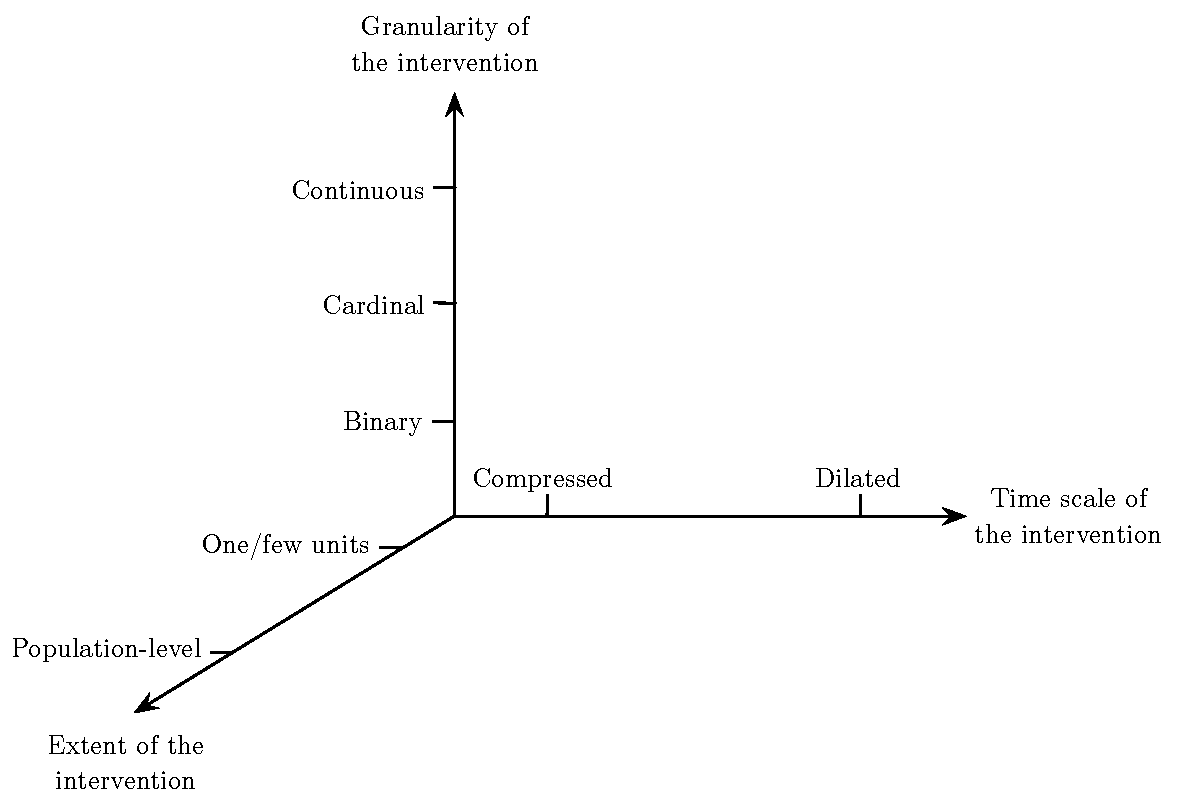
\includegraphics[width=1\textwidth]{exhibits/typology.pdf}
    \end{center}
    \caption{A typology of exogenous shocks. Notes. --- The `timescale of the 
    intervention' axis is a continuum; we annotate it with reference points
    in the interest of interpretability. }
    \label{fig:typology}
\end{figure}

The literature shows considerable variations regarding the first dimension, an 
\textit{exogenous shock's extent of intervention}. At one extreme of
the gamut, there are cases such as pilot or unique policies and rare
naturalistic or social events that affect one unit only.  For instance,  Nathan
\autocite*{nathan_2020} evaluates the causal impact of a flagship UK technology
cluster program that carries out an original `light-touch,' market-oriented
intervention. The policy under investigation --- which the author presents in
as an as-if random variation\footnote{Here is a passage from Nathan 
\autocite*{nathan_2020} where the author describes the empirical identification
strategy for the paper: \textit{``By 2010 Ministers were claiming
`something special' for the Inner East London cluster (Cameron, 2010; Osborne
and Schmidt, 2012). Other accounts depict policy origins as chaotic (Butcher,
2013; Nathan et al., 2019), and thus as good as random''} (page 5).} --- 
regards one cluster London solely (that is, `Tech City'). The study of Abadie 
and Gardeazabal \autocite*{abadie_gardeazabal_2003} is another example 
of an exogenous shock affecting one unit only. The authors use the terrorist 
conflict in the Basque Country as a case study to investigate the 
effect of conflict on regional GDP.

In other circumstances, exogenous shocks regard a fraction of the units included
in the reference population. Typical cases are empirical strategies that consider
the death of business or political leaders
\autocite[e.g.,][]{iyer_2010,bennedsen_et_al_2007,
nguyen_et_al_2010,nguyen_et_al_2014,johnson_et_al_1985,
lee_et_al_2020,ke2019439,kang20201300,jones_olken_2005,quigley_et_al_2017,
brown_et_al_2017}.  For instance, Iyer \autocite*{iyer_2010} uses the heirless
death of princes in the $19^{th}$ as a random variate accounting for the
transition of a district from the `indirect rule' to the `direct rule,' in which
British administrators collected taxes and administered local governance
themselves. The descriptive evidence reported in Iyer's work indicates twenty
districts out of 181 experience the heirless death.\footnote{Iyer considers the
twelve year timespan (1848 - 1856) where the Governor-General of India, Lord
Dalhousie, enacted a new policy Doctrine of Lapse, annexation would result from
the death of a ruler without a natural heir.} One of the studies included in our
systematic review of the literature \autocite{jia2020290} takes advantage of
SEC's pilot study consisting in exclusion of designated securities from the
operation of the `tick' test of Rule 10a-1(a) and any short sale price test rule
of any exchange or national securities association. Such a temporary
intervention resulted in a stock price risk surge for 512 firms belonging to the
Russell 3000 Index.

The other extreme of the gamut regards exogenous shocks that interest the whole
population of units. That could happen for different reasons. Sometimes,
governments introduce legal changes in a non-staggered manner, making new laws
binding at the same point in time for all firms located in the country.  An
example is Norway's gender quota policy, the shock central to the work of Matsa
and Miller \autocite*{matsa_miller_2013} on the implications of gender
composition in executive teams. Public limited companies had two years to comply
with the requirement of having at least 40 percent representation from each sex
on their board. According to the descriptive evidence reported in the study,
\textit{``nearly all firms complied by February 2008, and all did by April
2008''} (page 140). Exogenous shocks that affect the entire population of
reference can also emerge from events such as major catastrophes, pandemics,
recessions, or global-scale terrorist attacks. Examples are Corbo et al.
\autocite*{corbo2016323} and Vergne \autocite*{vergne20121027},
--- which rely on the variance created by 9/11 to investigate the change
of the airline industry and the boundaries of the global arm sector respectively
--- and Gupta et al. \autocite*{gupta2020802}, which draws on the Global 
Financial Crisis as a source of pressures for CFOs to report favorable results,

The second dimension of our topology --- 
intervention timescale --- emphasizes the timing with which an exogenous shock 
is presumed to affect a relationship or mechanism of interest. To clarify this dimension,
let us focus on one specific class of exogenous shocks: the death of
individuals occupying prominent positions in organization or fields. The finance
literature abounds of studies using sudden deaths amongst upper
echelons to address the overarching question `how do executives matter?'
\autocites[e.g.,][]{johnson_et_al_1985,nguyen_et_al_2014,nguyen_et_al_2010,
faccio_parsley_2009,salas_2010,fracassi_tate_2012,fee_et_al_2013,cho_et_al_2016,
dedman_et_al_2002,duchin_sosyura_2013,falato_et_al_2014}.
The intuition behind this body of work is that analyst and market reactions
to unanticipated executive turnover reveal the `net contribution'
of business leaders to shareholder value. As Nguyen 
and colleagues \autocite*[][]{nguyen_et_al_2014} note, stock price changes 
play a critical role as they

\begin{quote}
  \textit{
    ``reflect the expected incremental value of cash flows under the deceased
    executive net of this pay, relative to the expected incremental value of the
    replacement net of his pay.''
  }
  (page 3000)
\end{quote}

Since market expectations factor in broad arrays of time-variant elements (e.g.,
the search costs a firm may incur to fill the vacancy in), it is critically
important to pick up an appropriate time window within which stock prices foster
a \textit{ceteris paribus}, pre-post shock comparison. Nguyen and colleagues
\autocite*[][]{nguyen_et_al_2014} evaluate the impact of executives' sudden
death using 

\begin{quote}
  \textit{
    ``daily returns from the Center for Research in Security Prices (CRSP) for
    an 11-trading-day period around the death. The event day is defined as the
    trading day of the executive's death, or the first trading day following the
    death if it occurred on a nontrading day.''
  }
  (page 3000)
\end{quote}

Such a strand of finance literature stresses two aspects. First, sudden executive
deaths are essential sources of variance to estimate leaders' economic and 
financial impact.  Second, and more importantly for our typology,
there is a relatively tight time-frame where executive sudden deaths are
relevant; that is, they create exogenous shocks to address the question 
`how do executives matter?'

Studies across the fields of economics of science and sociology of science highlight a
different temporal pattern by which sudden deaths alter reference  processes or
mechanisms and, in turn, acquire relevance. Several articles
\autocites[e.g.,][]{azoulay_et_al_2019_b,azoulay_et_al_2019_a,khanna_et_al_2021,
aizenam_kletzer_2011,azoulay_et_al_2010,oettl_2012} take advantage of the 
start scientists' premature death to estimate better the spill-overs 
that emanate from collaboration. The seminal study of Azoulay and colleagues 
\autocite*{azoulay_et_al_2010} quantifies these spill-overs in terms of 
a scientist's differential of publications and research grants 
when collaborative ties collapse because of the death of an alter star 
scientist. Different to the finance literature, where executive deaths 
can create `instantaneous' change in expectations about a firm's 
future cash flows, Azoulay et al. \autocite{azoulay_et_al_2010}
consider a broad timespan to reveal the effect of exogenous shock. On the one 
hand, spill-overs can `roll over' after the death of a superstar collaborator. 
On the other hand, a scientist's research takes sufficient time to change. 
These elements seem to guide the choice of the authors to 
evaluate the effects of the shock in a fifteen-year time window
(see Figure \ref{fig:azoulay_et_al_2010}). At the same
time, they also account for the intertemporal variation of the superstar 
extinction effect:
 
\begin{quote}
  \textit{
    ``Following the superstar's death, the treatment effect increases
    monotonically in absolute value, becoming statistically significant three to
    four years after death. Two aspects of this result are worthy of note.
    First, we find no evidence of recovery --- the effect of superstar extinction
    appears permanent. Though we will explore mechanisms in more detail below,
    this seems inconsistent with a bereavement-induced loss in productivity.
    Second, the delayed onset of the effect makes sense because it plausibly
    takes some time to exhaust the productive potential of the star's last
    scientific insights. In addition, the typical NIH grant cycle is three to five
    years, and the impact of a superstar's absence may not really be felt until
    it becomes time to apply for a new grant.''
  }
  (page 568)
\end{quote}

\begin{figure}[!htbp]
    \begin{center}
      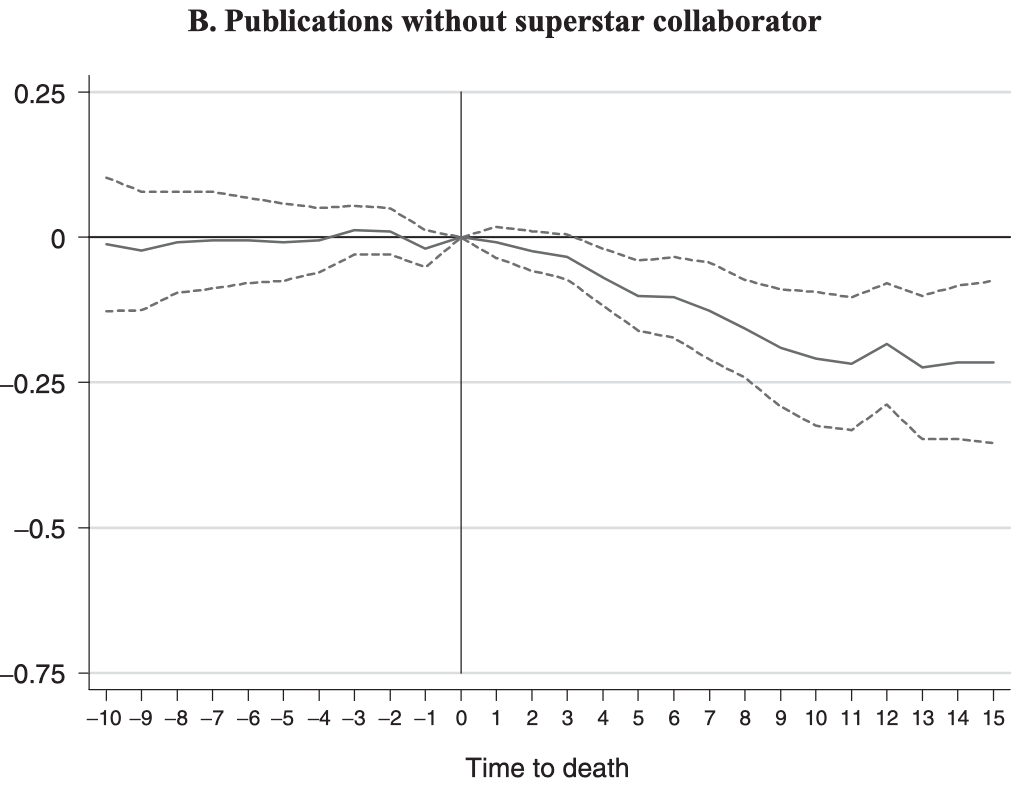
\includegraphics[width=0.75\textwidth]{exhibits/from_azoulay_et_al_2010.png}
    \end{center}
    \caption{A visualization included in Azoulay et al. 
    \autocite*[][]{azoulay_et_al_2010} clarifying the timescale of the 
    exogenous shock generated by the sudden death of a scientist's prominent
    collaborator. Notes. --- The figure, titled `Dynamics of Treatment Effects,'
    is reported a page 569. Here is the note describing the key aspects of the
    figure: ``The solid lines in the above plots correspond to coefficient
    estimates of conditional fixed effects quasi-maximum likelihood
    Poisson specifications in which the weighted publication output of a
    collaborator is regressed onto year effects, seventeen indicator
    variables corresponding to different age brackets, and interactions of the
    treatment effect with 27 indicator variables corresponding to eleven
    years before the year of death and prior, ten years before the year of death,
    nine years before the year of death, \ldots, fourteen years after the year of
    death, and fifteen years after the year of death and above (the indicator
    variable for treatment status interacted with the year of death is
    omitted).''}
    \label{fig:azoulay_et_al_2010}
\end{figure}

The third element of our typology regards the \textit{granularity of the 
intervention} that stems from the exogenous shock. The least granular 
intervention corresponds to a binary treatment that splits units into 
two experimental groups \textit{\'a la} Snow \autocite*{snow_1855}.
An intermediate level of granularity occurs when the exogenous shock 
is presumed to form more than two groups of units, each of which receives
a certain amount of treatment. For instance, the study included in our
review by Chen and Garg \autocite*{chen20181239} divides NBA teams into 
four strata: those not affected by a superstar injury (the control group) and 
those affected by a superstar injury implying `short,' `medium,' and `long' 
absence. Finally, an exogenous shock may create a continuous treatment. 
An example is  Drago and Galbiati's \autocite*{drago_galbiati_2012} paper
on social influence and criminal activity. The authors use the Collective 
Clemency Bill, the Italian Parliament approved in 2006, as an exogenous 
variation in the incentives to commit a crime:

\begin{quote}
  \textit{
    ``Upon approval of the bill, almost 22,000 inmates were released from Italian
    prisons. Of direct importance to the objective of this study, the bill
    stipulates that if a former inmate commits another crime within 5 years of
    their release from prison, they will be required to serve the residual
    sentence suspended by the pardon (varying from 1 to 36 months) in addition
    to the sentence for the new crime. In other words, the policy effectively
    transforms one month of an original sentence into an additional one month of
    sentence for future crimes committed at the individual level.''
  }
  (page 200)
\end{quote}

For Drago and Galbiati \autocite*{drago_galbiati_2012}, the shock does not
originate from the new law. Instead, it comes from the interaction between the
application of the law 
--- commuting actual sentences in expected sentences for forty percent of 
the Italian prison population --- and a prisoner's residual sentence at date of
release. Thanks to such an ingenious empirical strategy, the authors can show

\begin{quote}
  \textit{
    ``Peers' residual sentences greatly impact individual recidivism. The estimated
    impact of the average residual sentence of the group (excluding the
    individual himself) is comparable to the direct effect of the individual
    residual sentence. In particular, an average residual sentence of one
    additional month decreases the probability of being rearrested by 0.16
    percentage points. The considerable size of the indirect effects is
    consistent with a social multiplier of two in crime.''
  } (page 200)
\end{quote}


\section{Harnessing exogenous shocks: empirical strategy challenges}
\label{sec:harnessing_exogenous_shocks}

\noindent This section emphasizes the empirical strategy challenges that are more 
likely to arise across exogenous shocks with different features. Mainly,
we focus on three challenges: (1) the scope of applicability of Neyman's
Potential Outcome Framework; (2) the external validity of an average treatment 
effect; (3) interference between treated and control units, i.e., SUTVA 
violations. To do that, we map some ideal cases of exogenous shocks onto the typology presented in
the previous section (see Figure \ref{fig:comparative_static}).

Let us consider case $A$, where a binary intervention influences a significant
number of units by altering meaningful empirical relationships or theoretical
mechanisms in a short amount of time. That would be the typical `finance paper'
drawing on the variance generated by the sudden death of executives. For
instance, Nguyen and colleagues' \autocite*{nguyen_et_al_2014} paper is based on 149
sudden death events whose effects are presumed to manifest in a relatively short
timespan (i.e., eleven days). Such a case poses minimal concerns in terms of
empirical strategy.  First, the population of units contains a sufficient number of
controls to approximate the unobservable counterfactual (e.g., how a stock price
would have evolved absent the unanticipated executive turnover). Second, the
binary intervention variable is `well-behaved' and does not create range
restriction issues threatening the external validity of the empirical estimates.
Finally, the tight timescale of the intervention reduces the chances that
control units will be unintentionally treated or affected by treated units'
course of actions (that would be a vacancy chain at the executive
level involving both treated and control companies, which is unlikely in a
timespan such as the one Nguyen and colleagues \autocite*{nguyen_et_al_2014}
consider). 

\begin{figure}[!htbp]
    \begin{center}
      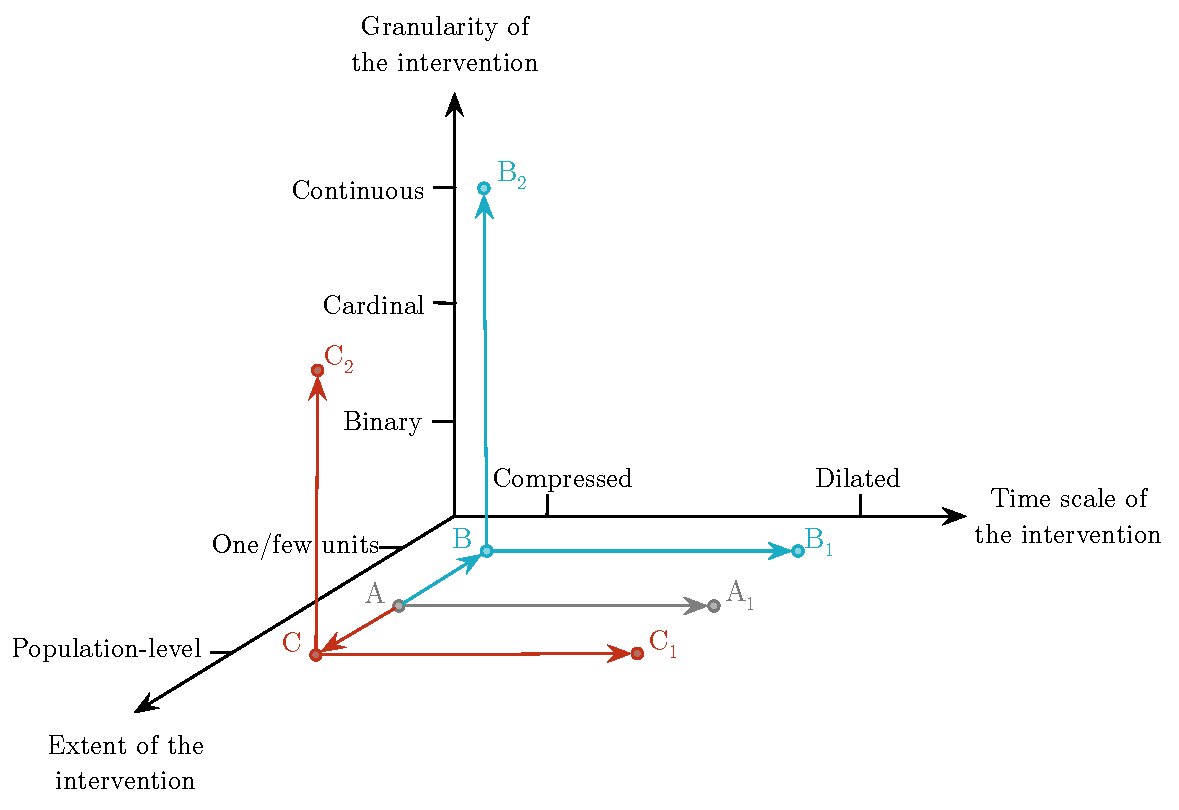
\includegraphics[width=1\textwidth]{exhibits/comparative_static.pdf}
    \end{center}
    \caption{Comparative static comprising ideal cases of exogenous shocks. 
    Notes. --- The key idea is that different cases present diverse 
    degrees of concern about (1) the scope of applicability of Neyman's
    Potential Outcome Framework; (2) the external validity of an average
    treatment effect; (3) interference between treated and control
    units.}
    \label{fig:comparative_static}
\end{figure}

Case $A_{1}$ differs from $A$ because of the timescale of the intervention,
which has a temporally dilated impact on the empirical relationships and 
theoretical mechanisms at the center of the study. Azoulay and colleagues'
\autocite*{azoulay_et_al_2010} paper on `superstar extinction' and knowledge
spill-overs is consistent with this case. The author's dataset contains 112
sudden, premature ends of elite life scientists, whose effects on circa five
thousand collaborators are modeled empirically over a fifteen-year timespan
(see Figure \ref{fig:azoulay_et_al_2010}). Similarly to $A$, chances are
significant the population will contain suited control cases and external
validity concerns will be least. However, interference issues may arise because
of the persisting impact of the shock.  For instance, the effects of super-star
extinction events may propagate over time through the social structure of
collaboration affecting treated units' collaborators supposed
to belong to the control group. Azoulay et al.  \autocite*{azoulay_et_al_2010}
propose supplemental analysis to deal with possible SUTVA violations, they
present in terms of the \textit{``problem of leakage through the coauthorship
network''} (page 579).

In general, relying on an exogenous shock such as $B$ poses external validity 
concerns. Plausible causes are generic range restriction issues --- i.e., a
treatment group with a limited variance --- and/or the presence of treated units
showing idiosyncratic features. The former may appear in studies with few
treated units \autocite[e.g.,][]{aizenam_kletzer_2011}.  The latter is common
when naturally-occurring events regard complex systems such as regions/countries
\autocite[e.g.,][]{abadie_gardeazabal_2003}, business platforms
\autocite[e.g.,][]{zhang2020}, or industrial clusters 
\autocite[e.g.,][]{nathan_2020}. Insofar as the population contains comparable
control units, an empirical strategy can still produce causal evidence in such a
scenario. However, the estimated effect is a local average treatment effect
(LATE) \autocite{imbens_2009} since it \textit{``it only characterizes causal
parameters for particular units''} \autocite[][page 290]{dunning_2012}. A
`cautious,' LATE interpretation of empirical estimates is --- if possible ---
even more critical in case $B_{2}$, where the increased granularity in the
treatment may exacerbate range restriction issues.\footnote{The key idea is that
the distribution of study variables conditional on different level of the
treatment may present significant sparsity.} Alternatively, the treated unit
might lack a match in the control group. Then, `Abadie's Comparative Case'
method 
\autocite{abadie_gardeazabal_2003,abadie_2021,abadie_et_al_2010,abadie_et_al_2015}
would be essential to create a synthetic counterfactual.\footnote{As Abadie
points out in his recent article \autocite*{abadie_2021}, the synthetic case
control method was originally proposed \textit{``with the aim to estimate the
effects of aggregate interventions, that is, interventions that are implemented
at an aggregate level affecting a small number of large units (such as a cities,
regions, or countries), on some aggregate outcome of interest'' (page 392).}}

Let us consider C. Sometimes, a naturally-occurring event's attributes and role 
\textit{vis \'a vis} the target research question impedes the identification
of a control group. In our review, some studies that
take advantage of the variance created by 9/11 for theorizing
\autocite{corbo2016323} or measurement purposes \autocite{vergne20121027}. 
In contrast, none uses 9/11 to create an exogenous shock study in the sense 
of a natural experiment. In other circumstances, the existence of surrogate 
populations allows researchers to bypass the problem of a total-spectrum 
exogenous shock. The gender quota study of Matsa and Miller 
\autocite*{matsa_miller_2013} is one of the most representative examples. 
The government of Norway applied the `40\% policy' in a non-staggered manner 
and made it mandatory for all public companies. The authors bypass
the lack of counterfactuals by adjusting their empirical strategy 
in two ways. First, they consider two surrogate populations, namely Norwegian
private firms and public firms located in Scandinavian countries (
textit{ex-ante}, similar to Norway in terms of culture and institutions). Second, they use 
a triple Difference-in-Difference estimator to create a composite counterfactual
that considers factors specific to the Norwegian 
economy and factors specific to comparable public companies. Compared with $C$,
cases $C_{1}$ and $C_{2}$ pose fewer constraints when identifying a 
control group. Under $C_{1}$, scholars can exploit the cross-section  
variance created by staggered policies. $C_{2}$ is consistent with studies 
using the variance generated by global events that, at least temporarily,
have heterogeneous effects across regions or countries.
Presumably, this case could become increasingly popular in the future 
as scholars use the Covid-19 pandemic as a source of variance in 
organizational practices (e.g., work from home).

In Figure \ref{fig:harnessing_exogeneous_shocks}, we use a decision tree to 
summarize the intuitions presented in this section of the paper. 

%\begin{landscape}
\begin{figure}[!htbp]
  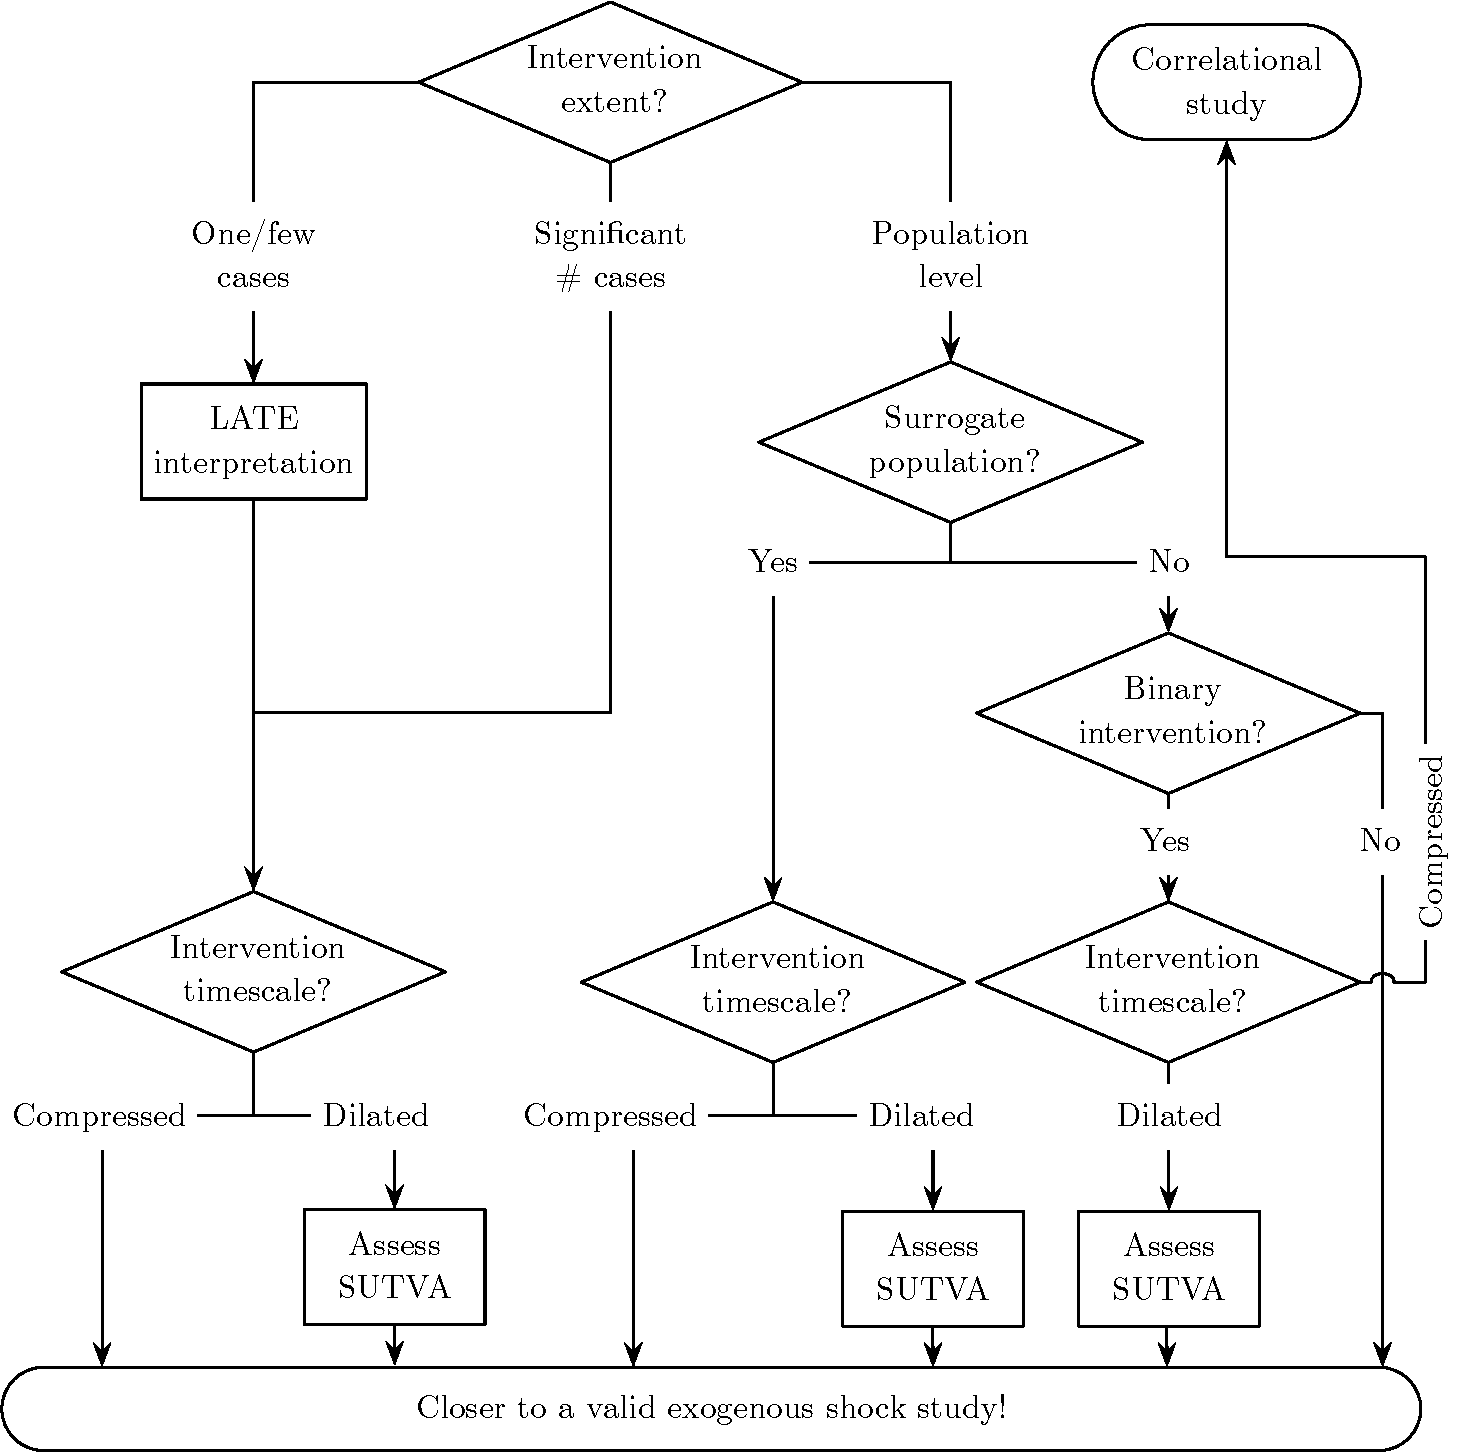
\includegraphics[width=1\textwidth]{exhibits/harnessing_exogenous_shocks.pdf}
  \caption{A decision tree to harness diverse exogenous shocks.}
  \label{fig:harnessing_exogeneous_shocks}
\end{figure}
%\end{landscape}

\section{Coda}
\label{sec:coda}

\noindent This paper aims to help authors and reviewers assess the 
validity of empirical strategies based on exogenous shocks. In the first arm of
this project, we have clarified the exogenous shock concept's boundaries and
ontological status. Mainly, we have stressed the idea that exogenous shocks do
not exist in the real world. Still, they emerge from the purposive association of
naturally-occurring events with concrete research questions.  As a
\textit{corollary}, it is not the intrinsic characteristics of a
naturally-occurring event that make a powerful exogenous shock study. In other
words, `relevant events' are not necessarily sudden, such as the death of a
business leader because of a hearth attack, uncontrollable, such as earthquakes,
or random, such as lotteries.  Instead, the relevance of a naturally-occurring
event is contingent on the empirical and theoretical problems at hand. 

In the second arm of the paper, we have argued that not all exogenous shocks are
born equal. Our original typology highlights three key features that 
differentiate exogenous shocks and help scholars anticipate which empirical 
strategy challenges are more likely to raise conditional on exogenous shock
types. Primarily, we have focused on three issues that have received 
limited or no consideration at all amongst leadership and management studies:
the scope of applicability of Neyman's Potential Outcome Framework; the 
external validity of the average treatment effect estimate --- i.e., the `LATE' 
interpretation of statistical estimates; the existence of treatment interference
issues resulting in SUTVA violations.

%% \item Environmental change - theory mapping
%% \item Temporal effects / timeline within which one expects the effects of the 
%% exogenous shock takes place
%% \item Scope to influence regulator's choices?
%% \item Time to react to regulator's choices?
%% \item Does a staggered adoption of legislative change correlate with 
%% admin/state-level features?
%% \item Exogenous shocks may have consequences that span multiple levels of 
%% analysis (e.g., sudden deaths of business owners)
%% \item Strategic purposes might lead the exogenous shock — entities that are 
%% treated might be passive — however, the policy maker may have incentives to 
%% treat certain entities
%% \item Conditional exogeneity (exogeneity within a statistical model sounds 
%% weird)
%% \item The nature of regulatory changes should be investigated from a 
%% multi-level perspective
%% \item Opportunities to marry the theoretical and empirical approaches to the 
%% study of shocks
%% \item Regulatory change — information, incentives, and capacity elements 
%% should be assessed before and after the introduction of the new law.
%% \item Scale of the shock and availabilities of counterfactuals
%% \item level of intervention and level of measurement
%% \item narrow spectrum interventions and idyosincratic interventions

%% --------------------------- Bibliography ---------------------------------
%\bibliographystyle{plainnat}
\section*{References}
\printbibliography[heading=none]
\end{refsection}

% -------------------------- Appendix --------------------------------------
%\begin{refsection}[references/sample.bib]
%
%\section{Appendix A --- Sample of studies}
%\label{sec:sampling}
%
%\setcounter{table}{0}
%\renewcommand{\thetable}{A\arabic{table}}
%\renewcommand{\thefigure}{A\arabic{figure}}
%
%!! Describe literature search !!
%
%\subsection{References}
%
%\printbibliography[heading=none]
%
%\end{refsection}

% ----------------------------- Closing ------------------------------------
\end{document}
